%&latex
% UF Sample ETD Main Document Fall 2016
% Documenting the conversion to xelatex compilation method
% Improved method of handling the single/multiple appendices issue
% Updated font calls to meet latest LaTeX standards


\documentclass[12pt,final,CPage]{ufthesis} %Use this line for Windows OS

% For those still using pdflatex and similar compilation methods - If you get a dvipdfm file not found error
% remove the dvipdfm and/or dvipdfmx options here and in the packages.tex file graphicx and hyperref packages and
% compile using Latex, Latex, Bibtex, Latex, Latex, XeLaTeX - this usually fixes
% the problem

%-------------------------------------C:\Program Files\MiKTeX 2.5\miktex----------------------------------%
% Preamble %

% Define Packages To be used and options NOTE: If you add any packages please add them before the hyperref package%
% here you define all the packages you wish to use in your paper, the ones shown are not all necessary,
% but all have purpose and can be very useful, so leave these as default and add packages as necassary
%\usepackage{graphicx}
%\usepackage[dvipdfmx]{graphicx}
\usepackage{amsmath}
\usepackage{amsthm}
\usepackage{algpseudocode}
%\usepackage{algorithm}
\usepackage{tabularx}
\usepackage{url}
%\usepackage[letterpaper,hmargin=1in,vmargin=1in]{geometry}
\usepackage{lscape}
%\usepackage{hanging}
\usepackage{longtable}
\usepackage{amsfonts}
\usepackage{amssymb}
%\usepackage[cmss]{sfmath} % Comment this line to use Times New Roman Math Typeface
\usepackage[cmbright]{sfmath} % Comment this line to use Times New Roman Math Typeface
\usepackage{subfigure}
\usepackage{rotating}
\usepackage{calc}
\usepackage{setspace}
\usepackage{ufenumerate}
\usepackage{latexsym}
%\usepackage{epsf}
\usepackage{epsfig}
\usepackage{euscript}
\usepackage[format=hang,justification=raggedright,singlelinecheck=0,labelsep=period]{caption}
%\usepackage[numbers,sort&compress]{natbib} %Use this set-up for numbered reference lists
\usepackage[authoryear]{natbib} %Use this set-up if you want an un-numbered reference list
%\usepackage{hypernat}



\usepackage[hyperfootnotes=false]{hyperref}
%\usepackage[dvipdfmx,hyperfootnotes=false]{hyperref}
%\usepackage[dvips,hyperfootnotes=false]{hyperref}
\hypersetup{colorlinks=true,linkcolor=blue,anchorcolor=blue,citecolor=blue,filecolor=blue,urlcolor=blue,bookmarksnumbered=true,pdfview=FitB} %
% % %DO NOT PLACE ANY PACKAGES AFTER THE HYPERREF SET UP


%\def\UrlFont{\rmfamily} %use this line for Times New Roman
\def\UrlFont{\sffamily} %use this line for CMSS

%\allowdisplaybreaks  % % This command allows equation arrays and similar environments
% % % to break across pages to improve text flow - use only if needed.

% Prevent figures, tables or algorithms from using a separate page or column alone
\renewcommand{\topfraction}{0.85}
\renewcommand{\textfraction}{0.1}
\renewcommand{\floatpagefraction}{0.75}

% *** Do not adjust lengths that control margins, column widths, etc. ***
% *** Do not use packages that alter fonts (such as pslatex).         ***
% There should be no need to do such things with IEEEtran.cls V1.6 and later.
% correct bad hyphenation here
%\hyphenation{op-tical net-works semi-C:\Program Files\MiKTeX 2.5\miktexconduc-tor}

%------------------------------------------%

% Extra commands or misc formatting such as page alignment or output paper-size commands

%\include{extraparameters}

%------------------------------------------%

% Set your personal and paper information
\SetFullName{Anurag Peshne}%
\SetThesisType{Thesis}
\SetDegreeType{Master of Science}
\SetGradMonth{August}%
\SetGradYear{2018}%
\SetDepartment{Computer \& Information Science \& Engineering}%
\SetChair{Beverly A. Sanders}%
%\SetCochair{John W. Carver III}%uncomment this line and enter the name of your cochair inside the braces if you have one.
%If you have a cochair there two places in the ufthesis.cls file that will need to be uncommented as well
%In the "getting personal information" section about line 630
%And the "Abstract" Section around line 556
% Type your title here in all CAPS %
\SetTitle{ENHANCEMENTS TO LOOPING CONSTRUCTS BY PREFETCHING AND EXPLOITING GPU}


%------------------------------------------%

% user defined commands in order to geC:\Program Files\MiKTeX 2.5\miktexnerate new commands, macros, and redefine default commands %
% user defined commands %
% Here is where you define optional commands such as macros, new commands,
% and new environments to be used in your paper

% optional command to prevent a word from breaking across a line %
\hyphenchar\font=-1


% Commands to produce proper bullet list
\newlength{\widthOfItem}
\let\Itemize=\itemize
\let\endItemize=\enditemize
\renewenvironment{itemize}{%
	\begin{Itemize}
		\setlength{\itemsep}{0.5\baselineskip}
		\setlength{\labelwidth}{2em}
		\setlength{\listparindent}{.32in}%
		\setlength{\leftmargin}{.32in}
		\setlength{\rightmargin}{0in}
		\settowidth{\widthOfItem}{\labelitemi}
		\setlength{\labelsep}{\leftmargin-\widthOfItem}
		\renewcommand{\labelitemii}{--}
		\singlespacing}{%
	\end{Itemize}}

% shortcut for setting up inserting \prime command in mathmode to avoid errors %
\newcommand{\p}{^{\prime}}

% shortcuts for prime color text
\newcommand{\red}{\textcolor[rgb]{1.00,0.00,0.00}}
\newcommand{\green}{\textcolor[rgb]{0.00,1.00,0.00}}
\newcommand{\blue}{\textcolor[rgb]{0.00,0.00,1.00}}

% Shorcut commands for mathmatical formulas %

\newcommand{\latex}{\LaTeX 2\ensuremath{\epsilon}}

% THEOREM Environments ---------------------------------------------------
%These environments are provided as a convenience - feel free to modify if needed

\newtheorem{theorem}{Theorem}[chapter]%To link the theorem to each chapter uncomment the chapter option
\newtheorem{lemma}{Lemma}%[theorem]% To link each lemma to a theorem uncomment the theorem option
\newtheorem{corollary}{Corollary}%[theorem]% To link each corollary to a theorem uncomment the theorem option
% to link a corollary to a chapter change the theorem option to chapter
\newtheorem{definition}{Definition}%[chapter] %the same is true for both definitions and assumptions
\newtheorem{assumption}{Assumption}%[chapter] %
\newtheorem{proposition}{Proposition}[chapter]
\newtheorem{algorithm}{Algorithm}[chapter]


%These were some user commands I've run across that I thought some might want to incorporate into their work
%\newcommand{\bdm}{
 %   \begin{displaymath}}

%\newcommand{\edm}{
%    \end{displaymath}}

%\newcommand{\be}{
%    \begin{equation}}

%\newcommand{\ee}{
%    \end{equation}}

%\newcommand{\bea}{
 %   \begin{eqnarray}}

%\newcommand{\eea}{
%    \end{eqnarray}}


%-------------------------------------------------------------------------------------------------------%

% Begin Main Part of Document %

\begin{document}


 % % % % % % % % % % % % % % % % % % % % % % % % % % % % % % % % % % % % % %
 % Remember - You MUST get a .bst file that matches the Journal in your
 % field that you choose as your Reference example
 % NONE of these examples will satisfy the Graduate Editorial Office
 % if they don't match your Journal example!!!!
 % NOTE: If you use a numbered reference system and your references
 % are set in parentheses rather than brackets you need to select the
 % Natbib option "numbers sort and compress" in the packages.tex file
 % % % % % % % % % % % % % % % % % % % % % % % % % % % % % % % % % % % % % %


 %Note that the path separator is a forward slash NOT a back slash
 %Place YOUR .bst file in the bst folder and use that filename (without the .bst extension)
 % as your Bibliography Style file

%\bibliographystyle{bst/abbrv}
%\bibliographystyle{bst/abbrvnat}
%\bibliographystyle{bst/abbrvurl_uf}
%\bibliographystyle{bst/alphaurl_uf}
%\bibliographystyle{bst/apa-good}
%\bibliographystyle{bst/Chicago_Web}
%\bibliographystyle{bst/ecology_web}
\bibliographystyle{bst/IEEEtran}
%\bibliographystyle{bst/mla_web}
%\bibliographystyle{bst/mla-good}
%\bibliographystyle{bst/plainnat}
%\bibliographystyle{bst/plainurl_uf}
%\bibliographystyle{bst/Science_Web}
%\bibliographystyle{bst/uf_econ}
%\bibliographystyle{bst/uffull}
%\bibliographystyle{bst/ufinit}
%\bibliographystyle{bst/unsrtnat}
%\bibliographystyle{bst/unsrturl_uf}
%\bibliographystyle{bst/plain}
%\bibliographystyle{bst/ufinit}
%\bibliographystyle{bst/plainurl_uf}


%-----------------------------------------------------------------------%

\maketitle % % % % Creates the Title page from the information entered in userinfo.tex
\makecopyright

%------------------------------------------%

\dedication{% Add your text for the dedication here between the center tags
%\addvspace{4.25in}
%\begin{center}%\singlespacing
\vspace{-20 mm}
I dedicate this to everyone that helped revamp this template. Aliquam molestie sed urna quis convallis. Aenean nibh eros, aliquam non eros in, tempus lacinia justo. In magna sapien, blandit a faucibus ac, scelerisque nec purus. Praesent fermentum felis nec massa interdum, vel dapibus mi luctus. Cras id fringilla mauris. Ut molestie eros mi, ut hendrerit nulla tempor et. Pellentesque tortor quam, mattis a scelerisque nec, euismod et odio. Mauris rhoncus metus sit amet risus mattis, eu mattis sem interdum.\\
%\end{center}
} % %Creates the dedication - if your dedication is more than a single line
% % % % % % % % % % % % % % % % % %you will need to reduce the vspace amount to keep the text centered verticlly
% % % % % % % % % % % % % % % % % %optional - comment or delete if you are not dedicating to anyone,

%------------------------------------------%

% Make sure to keep the text within the brackets and the output should turn out correct
\acknowledge{%
Thanks to all the help I have received in writing and learning about
this tutorial. Acknowledgments are required and must be written in paragraph form. This mandates at least three sentences. }
 % % % %Required - There is no requirement to acknowledge a particular person
% % % % % % % % % % % % % % % % %but you must acknowledge someone (funding source, committee chair, spouse)?

%------------------------------------------%

% This file includes the file which creates the table of contents %
% This creates your table of contents, list of figures, and list of tables
% the pdfbookmark line adds the word to the bookmarks of the pdf without adding it to the TOC itself
\pdfbookmark[0]{TABLE OF CONTENTS}{tableofcontents}
\tableofcontents %
\listoftables %
%\setcounter{lofdepth}{2}
\listoffigures %

% Produced list of abbreviations or symbols %
%\printindex[keylist]{KEY TO ABBREVIATIONS}{KEY TO ABBREVIATIONS}{}
%\printindex[mathlist]{KEY TO SYMBOLS}{KEY TO SYMBOLS}{%
%The list shown below gives a brief description of the major mathematical symbols defined in this work. For each
%symbol, the page number corresponds to the place where the symbol is first used.} %
 %This file creates the Table of Contents, List of Figures, and List of Objects (if any)
% % % % % % % %delete or comment the file you want to remove

%------------------------------------------%

%%This is an optional file. A list of abbreviations is NOT even suggested.
%%Best practice is to define the item the first time it is used in the document

%%%-----------List of Symbols, Nomenclature or Abbreviation--------

%% Please note: a list of Symbols, terms, acronyms, etc. is not usually the best practice.
%% More often you should simply define an abbreviation the first time it is used.
%% If you DO need to include a list like this please notice that it must be paginated manually
%% by breaking it up into page size tables. Longtable will not wrap the definition properly if
%% it extends to a second line and a similar issue is encountered when the tabbing environment
%% is used. If you have a better way of meeting the Editorial Office requirements I'd love to hear about it.

\chapter*{LIST OF SYMBOLS, NOMENCLATURE, OR ABBREVIATIONS} \addcontentsline{toc}{chapter}{LIST OF SYMBOLS} %Start
%writing here. This is optional.
\singlespacing
\begin{tabular}{l p{5in}} %if the terms in the first column are longer than 1.4 inches reduce the number 5 appropriately
$\sum$ & Denotes the summation of a series of terms\\
\\%This adds the single space between definitions (required)
$\bigcap$ & A really big bigcap\\
\\
fractal & A geometric pattern that is repeated at ever smaller
scales to produce irregular shapes and surfaces that cannot be represented by classical
geometry. Fractals are used especially in computer modeling of irregular patterns and structures in nature.}\\
\\
polynomial & (in one variable) an expression consisting of the sum of two
or more terms each of which is the product of a constant and a
variable raised to an integral power: $ax^2 + bx + c$ is a
polynomial, where $a, b,$ and $c$ are constants and $x$ is a
variable.}\\
\\
$\sum$ & Denotes the summation of a series of terms\\
\\
$\bigcap$ & A really big bigcap\\
\\
fractal & A geometric pattern that is repeated at ever smaller
scales to produce irregular shapes and surfaces that cannot be represented by classical
geometry. Fractals are used especially in computer modeling of irregular patterns and structures in nature.}\\
\\
polynomial & (in one variable) an expression consisting of the sum of two
or more terms each of which is the product of a constant and a
variable raised to an integral power: $ax^2 + bx + c$ is a
polynomial, where $a, b,$ and $c$ are constants and $x$ is a
variable.}\\
\\
$\sum$ & Denotes the summation of a series of terms\\
\\
$\bigcap$ & A really big bigcap\\
\\
fractal & A geometric pattern that is repeated at ever smaller
scales to produce irregular shapes and surfaces that cannot be represented by classical
geometry. Fractals are used especially in computer modeling of irregular patterns and structures in nature.}\\
\\
polynomial & (in one variable) an expression consisting of the sum of two
or more terms each of which is the product of a constant and a
variable raised to an integral power: $ax^2 + bx + c$ is a
polynomial, where $a, b,$ and $c$ are constants and $x$ is a
variable.}\\

\end{tabular}

\begin{tabular}{lp{5in}}
$\sum$ & Denotes the summation of a series of terms\\
\\
$\bigcap$ & A really big bigcap\\
\\
fractal & A geometric pattern that is repeated at ever smaller
scales to produce irregular shapes and surfaces that cannot be represented by classical
geometry. Fractals are used especially in computer modeling of irregular patterns and structures in nature.}\\
\\
polynomial & (in one variable) an expression consisting of the sum of two
or more terms each of which is the product of a constant and a
variable raised to an integral power: $ax^2 + bx + c$ is a
polynomial, where $a, b,$ and $c$ are constants and $x$ is a
variable.}\\
\\
$\sum$ & Denotes the summation of a series of terms\\
\\
$\bigcap$ & A really big bigcap\\
\\
fractal & A geometric pattern that is repeated at ever smaller
scales to produce irregular shapes and surfaces that cannot be represented by classical
geometry. Fractals are used especially in computer modeling of irregular patterns and structures in nature.}\\
\\
polynomial & (in one variable) an expression consisting of the sum of two
or more terms each of which is the product of a constant and a
variable raised to an integral power: $ax^2 + bx + c$ is a
polynomial, where $a, b,$ and $c$ are constants and $x$ is a
variable.}\\
\\
$\sum$ & Denotes the summation of a series of terms\\
\\
$\bigcap$ & A really big bigcap\\
\\
fractal & A geometric pattern that is repeated at ever smaller
scales to produce irregular shapes and surfaces that cannot be represented by classical
geometry. Fractals are used especially in computer modeling of irregular patterns and structures in nature.}\\
\\
polynomial & (in one variable) an expression consisting of the sum of two
or more terms each of which is the product of a constant and a
variable raised to an integral power: $ax^2 + bx + c$ is a
polynomial, where $a, b,$ and $c$ are constants and $x$ is a
variable.}\\
\\
\end{tabular}
\doublespacing




%------------------------------------------%
% This line adds the word CHAPTER to the TOC just before the listing of the chapter and subsections begins
\addtocontents{toc}{\protect\addvspace{10pt}\noindent{CHAPTER}\protect\hfill\par}{}% This extra line adds the word CHAPTER to the table of contents %
\phantomsection
% Write in only the text of your abstract, all the extra heading jargon is automatically taken care of
\begin{abstract}
  The Super Instruction Architecture (SIA) is a parallel programming environment
  engineered to work on large blocks of floating point numbers. Looping constructs
  \texttt{do} and \texttt{pardo} are one of the most important constructs in Super
  Instruction Assembly Language (SIAL) since they allow the programmer to work
  with an individual block. To improve the runtime performance of the looping constructs,
  two techniques are used: improving GPU utilization and prefetching blocks to
  hide network latency.\\

  In the previous versions, the domain programmer was needed to manually transfer blocks between main memory
  and GPU memory as well as to mark parts of SIAL code to be executed on GPU. Copying data
  between GPU memory and main memory is costly and have a high impact on overall
  performance of GPU execution. Automatic memory management is provided
  and various techniques are implemented to reduce and in some cases eliminate
  GPU memory and main memory transfer cost.\\

  There is a common code pattern in SIAL to request a block of data followed by
  computation on that block. This pattern makes inefficient use of network
  and compute resources, since one remains underutilized while the other is being used.
  Deterministic request for blocks has been exploited
  to implement prefetching to optimally utilize the network resources during the time
  computational resources have blocked the control flow.\\

  Various experiments have been conducted to evaluate the effect of change of various
  parameters on GPU utilization, prefetching, \texttt{wait\_time} and overall
  computation time.
\end{abstract}
 %The abstract is created using this file and userinfo.tex
% % % % % % % % % % %If you have a c-chair you must uncomment that line in userinfo.tex AND find the
% % % % % % % % % % %co-chair lines in ufthesis.cls and un-comment those as well

%-----------------------------------------------------------------------%

% This section encompasses the main body of the paper from all the content through to the biographical sketch

% Chapters to be included (more can be added by creating a new chapter#.tex %
% file and then implementing the \inlcude{chapter#.tex} command as seen below %
\chapter{INTRODUCTION TO THESIS}\label{intro}
The Super Instruction Architecture (SIA) is a parallel programming environment
originally designed for problems in computational chemistry involving complicated
expressions defined in terms of tensors. Tensors are represented by
multidimensional arrays which are typically very large. The SIA consists of a
domain specific programming language, Super Instruction Assembly Language
(SIAL), and its runtime system, Super Instruction Processor. An important
feature of SIAL is that algorithms are expressed in terms of blocks or
multidimensional arrays rather than individual floating point numbers.

\section{Introduction to Issues with Working with GPUs}
In ACESIII, the previous version of ACES, programmer had to explicitly deal with managing
the memory transfer between GPU and CPU and marking regions well suited for execution
on GPU. In ACES4, managing memory transfer is done automatically by the runtime.
This is implemented by tracking block changes using version numbers.

Still there is need for SIAL programmer to decide which portion of the SIAL code
is well suited for execution on GPU. Transferring data between GPU and CPU is
expensive and can dominate the total time spend in computation. Hence this is not
a trivial decision to make since the programmer has to minimize time spend in
total memory transfers. This in turn depends on various factors such as
size of the block and number of instructions in the code block supported on GPU. Judging
based on size of block is itself difficult because it depends on the type of GPU available
at runtime. Larger blocks need more time to transfer between GPU and CPU, but at
same time the difference in time taken to operate on blocks by GPU and CPU grows
exponentially with the size of the block. And lastly, same programs are used to
calculate different results by supplying different data files. A portion of code
which executed faster on GPU for certain block size may in fact execute slower
than on CPU for smaller block size if the gain in time by executing on GPU cannot
compensate for the transfer time.

\section{Introduction to Issue of Data Transfer from Server}
In SIAL, looping constructs are the only way to work with individual blocks.
Typical work~flow of SIAL includes requesting a block of larger array from server,
processing the block, compute resulting block and send it back to the server. Though
the operation of requesting block from server is non blocking, subsequent operations
in the loop block until MPI transfer is completed. To amortize the cost of network
transfer, prefetching has been implemented which does the transfer concurrently
with the block processing. By prefetching the anticipated blocks that would be
needed in next iteration of loop, the wait~time for block can be reduced and
in some cases completely eliminated.

\section{Organization of the Thesis}
Chapter 2 presents related literature regarding efforts made to exploit GPU in
SIA as well as other programming models and the technique of prefetching to hide
latency in accessing data. Then an introduction to background of this thesis,
including architecture and implementation of SIA and ACES4, is presented in chapter~3.
Chapter 4 describes the problem and solution of optimizing use of GPU to execute SIAL
code; the design and implementation of eager-pushing of blocks and dynamic
determination of suitable code block for execution on GPU is presented in
chapter 5. Chapter 6 states the results of the benchmarks and experiments. And
finally, chapter 7 presents conclusion of this thesis and future works. % introduction
\chapter{BACKGROUND: SUPER INSTRUCTION ARCHITECTURE} \label{background}

This chapter introduces the SIA, ACES4, block-based
programming, the design of workers and servers, SIAL, parallel looping constructs
and design of GPU implementation.

\section{SIA}
The SIA is a special purpose, domain agnostic, parallel programming framework which
is engineered for solving computation on very large, possibly sparse, multidimensional
arrays. Programmer using SIA expresses the computation in terms of blocks of multidimensional arrays
and instructions which operate on these blocks.

In contrast, in conventional programming languages a computation is described in terms of individual floating point
number and operations which work on these individual numbers. Aggregating
individual numbers into blocks results in better performance and higher utilization
of resources. However, this adds considerable complexity to programs since now
the programmer has to deal with tedious and error prone index arithmetic.

Algorithms in SIA can be directly expressed in terms of
blocks. This gives the performance benefits of using blocks and at the same time relieves
programmer from error-prone work of dealing with indices and looping. Expressing
computations in terms of blocks has multiple performance advantages: moving data
blocks is more efficient since it has less overhead per individual number
and runtime can overlap computation and network operation since transferring these
blocks will take significant time, resulting in better overall utilization of resources.
There is an added advantage of expressing computation in terms of blocks in a parallel
framework: the work can be distributed among participating nodes in a natural
way. This is essential when multidimensional arrays are too large to hold in
physical memory of a single processor.

\section{Overview of ACES}
ACES4 is an implementation of the SIA for chemical computation. It has been executed
on a variety of architectures but is specially optimized to enable
calculations on leadership-class supercomputers. Using ACES4, computational chemists
try to find approximate solutions to the electronic Schrödinger equation using Coupled cluster
methods. There exist other methods to calculate approximate solutions but Coupled
cluster methods, although computationally expensive, are one of the most accurate methods.
The chemical computation done using ACES4 uses data of high dimensions. A typical calculation in this domain
takes as input the geometry of a molecular system and a choice of single
particle orbitals as the basis to expand the many-electron quantum-mechanical wave
function. The complex algorithms, which produce properties of the molecular
system, can easily require arrays of double precision floating point upto
several hundred Gigabytes. Of these arrays, at least three need rapid access and
are usually stored in RAM, the rest that are used less frequently can be stored
on disk. The SIA architecture is very suitable for these kinds of calculations since
the workers can work on parts of array concurrently and the servers can swap out
less frequently used arrays to disk.

\section{Architecture of SIA}\label{siaarch}
The SIA can execute instructions in parallel over multiple processors. It can be
deployed and scaled on multiple nodes in a high performance computing cluster
using MPI for internode communication.

The SIA supports arrays of size greater than the combined memory of all processors
involved in computation by providing the facility of storing the chunks which are
not \textit{hot}, that is the chunks which are not going to be used soon, on
larger, although slower, memory on hard drives. This swapping of blocks is automatic
and transparent to the programmer. To facilitate the movement of data among
processing units and swapping out blocks to hard drives, SIA divides available
processors into two groups: workers and servers --- the workers are responsible for
actual execution of instructions on the blocks, while the servers make sure blocks
are served to and from the workers.

\section{SIAL}
SIAL is a programming language provided for expressing problems of the target
domain. The idea behind SIAL is to keep the domain issues separate from
the platform issues. SIAL programs are written by the domain experts
whereas the intricacies involved in execution of SIAL programs, like distribution of
data, parallel execution, memory management, runtime optimizations, are handled
by computing experts.

SIAL, in addition to providing programmers with conventional constructs such as
conditional constructs, looping constructs, procedures, way to import other SIAL
programs like general purpose programming language, also provides special parallel looping construct and a way
to define domain-specific block operations or \textit{super instructions}. It
has several common block operations built in. The
parallel looping construct, \texttt{pardo}, loops over multiple indices and
distributes loop iterations to different processors. This construct is of special
interest to us since the optimizations done using GPUs are mostly done in the
interpretation of this looping construct.

As mentioned above, domain experts can write their own domain-specific
super instructions which take in single or multiple blocks and output a resulting block. These
instructions can be written in any general purpose programming language by following
the SIAL calling interface. There are implementations of super instructions in
C++ and Fortran in ACES4. Since these languages are much
closer to the hardware, these super instructions can be written in a very
optimized way. Further more, this facility can be exploited to port the super instructions to
other computing devices such as GPU by writing these super instructions using
Nvidia CUDA.

\subsection{SIAL Interpreter}
The SIA includes a SIAL compiler which translates human-readable SIAL text to
machine friendly bytecode. This bytecode is interpreted by SIAL interpreter.
Since this interpretation happens at runtime, the interpreter is able to optimize the
execution based on resources available at runtime. If interpreter finds GPU
accessible, it may execute some part of the SIAL program on GPU and if it
doesn't find it, then it can automatically fallback to CPU. Similarly, there are
various optimizations implemented which depend on the amount of physical memory
present on the processor.

\section{Block Structure}
As described above, instead of processing data as a single floating point
number, the SIA processes blocks of floating point numbers. These blocks are chunks
of even larger multidimensional arrays. Blocks are represented inside SIAL
interpreter using the \texttt{Block} class. The SIA supports heterogeneous computing
using other computing devices such as GPUs. Since GPUs have their own device memory
which is separate from main processor memory, there is a facility in the
\texttt{Block} class to represent the block memory in other
computing devices. Along with member attributes which represent block metadata
and member functions which act on the block, the Block class has pointers to
the memory location on each computation unit: CPU, GPU and support for more
computing device such as Intel Xeon Phi.

The \texttt{Block} class, depending upon the active computing device, will return the
appropriate device memory address. There is also logic build into the \texttt{Block}
class to automatically synchronize memory for various devices, so that if one
device modifies the block and then in next instruction, another device wants
to read the block, the block memory will be automatically synchronized and the
next device will read updated memory. This is done by maintaining version numbers
for each memory and then updating the memory based upon the version numbers when
it is accessed.

\section{Executing Super Instructions on GPU}
There are two ways in which GPUs are exploited in the SIA to obtain high concurrency.
First, the super instructions can be written in CUDA.
Using CUDA, these instructions can make use of low-level hardware
features and domain knowledge to fine-tune the implementation. Secondly, some of
the general purpose block operations such as matrix multiplication, addition,
scaling, tensor contraction for GPU are builtin the interpreter
itself. These operations can be imported from highly optimized libraries such as
Nvidia CuBLAS.

The SIAL interpreter takes care of executing GPU or CPU implementation of an
operation based upon availability of implementations and other factors such as
the size of input and output. % related work
\chapter{BACKGROUND: SUPER INSTRUCTION ARCHITECTURE} \label{background}

This chapter introduces the SIA, ACES4, block-based
programming, the design of workers and servers, SIAL, parallel looping constructs
and design of GPU implementation.

\section{SIA}
The SIA is a special purpose, domain agnostic, parallel programming framework which
is engineered for solving computation on very large, possibly sparse, multidimensional
arrays. SIA expresses the computation in terms of blocks of multidimensional arrays
and instructions, which operate on these blocks. This way of expressing a computation
is different from conventional programming
languages, wherein computation is described in terms of individual floating point
number and operations which work on these individual numbers. Aggregating
individual numbers into blocks results in better performance and higher utilization
of resources. However, this adds considerable complexity to programs since now
the programmer has to be careful of the index arithmetic and designing algorithms to loop
over entire blocks. Algorithms in SIA can be directly expressed in terms of
blocks. This gives the performance benefits of using block and at the same time relieves
programmer from error-prone work of dealing with indices and looping. Expressing
computation in terms of blocks has multiple performance advantages: moving data in terms
of blocks is more efficient since it has less overhead per individual number
and runtime can overlap computation and network operation since transferring these
blocks will take significant time, resulting in better overall utilization of resources.
There is an added advantage of expressing computation in terms of blocks in a parallel
framework, that the work can be distributed among participating nodes in a natural
way.

Since these multidimensional arrays can be too
large to hold in physical memory of a single processor, they are broken into
blocks or super numbers. These super numbers are used as input to special instructions
written to operate on blocks instead of floating point numbers. These
instructions are called as super instructions. Section~\ref{siaarch} describes how
these blocks are managed among participating processors.

SIA can execute instructions on blocks in parallel on multiple processors. To
facilitate movement of blocks among parallel execution units, server-client
architecture is used. SIA provides SIAL, a block-oriented domain specific
language (DSL), which supports expressing algorithms using blocks and a way
to write super instructions, which are domain specific, in an optimized way. The
following sections describe details of working of server-client architecture,
SIAL, and constructs in it.

\section{Architecture of SIA}\label{siaarch}
SIA can execute instructions in parallel over multiple processors. It can be
deployed and scaled on multiple nodes in a high performance computing cluster
using MPI for internode communication. Since the
multidimensional arrays involved in the calculations can be extremely large for
the memory of a single processor, SIA divides the arrays into chunks of
manageable sizes. These chunks are distributed to different processors and the
processors can work on these chunks concurrently.

SIA supports arrays of size greater than the combined memory of all processors
involved in computation by providing the facility of storing the chunks which are
not \textit{hot}, that is the chunks which are not going to be used soon, on
larger, although slower, memory on hard drives. This swapping of blocks is automatic
and transparent to the programmer. To facilitate the movement of data among
processing units and swapping out blocks to hard drives, SIA divides available
processors into two groups: workers and servers --- the workers are responsible for
actual execution of instructions on the blocks, while the servers make sure blocks
are served to and from the workers. The division of the number of the servers versus the number
of the workers is chosen by SIA but can be overridden by passing command line
arguments.

\section{SIAL}
SIAL is a programming language provided for expressing problems of the target
domain. The idea behind SIAL is to keep the domain problem separate from
platform problem. SIAL programs are written by the domain experts
whereas the intricacies involved in execution of SIAL programs, like distribution of
data, parallel execution, memory management, runtime optimizations, are handled
by computing experts.

SIAL, apart from providing programmers with conventional constructs such as
conditional constructs, looping constructs, procedures, way to import other SIAL
programs like general purpose programming language, also provides special parallel looping construct and a way
to define domain-specific block operation or \textit{super instruction}. It
has several common block operations built in. The
parallel looping construct, \texttt{pardo}, loops over multiple indices and
distributes blocks to different processors. This construct is of special
interest to us since the optimizations done using GPUs are mostly done in the
interpretation of this looping construct.

As mentioned above, domain experts can write their own domain-specific
super instructions which take in single or multiple blocks and output a resulting block. These
instructions can be written in C, C++ or Fortran. Since these languages are much
closer to the hardware, these super instructions can be written in a very
optimized way. Further more, this facility can be exploited to port the super instructions to
other computing devices such as GPU by writing these super instructions using
Nvidia CUDA.

\subsection{SIAL Interpreter}
SIA consists of SIAL compiler which translates human-readable SIAL text to
machine friendly bytecode. This bytecode is interpreted by SIAL interpreter.
Since this interpretation happens at runtime, the interpreter is able to optimize the
execution based on resources available at runtime. If interpreter finds GPU
accessible, it may execute some part of the SIAL program on GPU and if it
doesn't find it, then it can automatically fallback to CPU. Similarly, there are
various optimizations implemented which depends on the amount of physical memory
present on the processor.

\section{Block Structure}
As described above, instead of processing data as a single floating point
number, SIA processes blocks of floating point numbers. These blocks are chunks
of even larger multidimensional arrays. Blocks are represented inside SIAL
interpreter using \texttt{Block} class. SIA supports heterogeneous computing
using other computing devices such as GPUs. Since GPUs have their own device memory
which is separate from main processor memory, there is a facility in
\texttt{Block} class to represent the block memory in other
computing devices. Along with member attributes which represent block metadata
and member functions which act on the block, the Block class has pointers to
the memory location on each computation unit: CPU, GPU and support for more
computing device such as Intel Xeon Phi.

The \texttt{Block} class depending upon the active computing device will return the
appropriate device memory address. There is also a logic build into the \texttt{Block}
class to automatically synchronize memory for various devices, so that if one
device edits the block and then in next instruction, another device wants
to read the block, the block memory will be automatically synchronized and the
next device will read updated memory. This is done by maintaining version numbers
for each memory and then updating the memory based upon the version numbers when
it is accessed.

\section{Executing Super Instructions on GPU}
There are two ways in which GPUs are exploited in SIA to obtain high concurrency.
First, the super instructions can be written in CUDA.
Using CUDA, these instructions can make use of low-level hardware
features and domain knowledge to fine-tune the implementation. Secondly, some of
the general purpose block operations such as matrix multiplication, addition,
scaling, tensor contraction can be implemented for GPU in the interpreter
itself. These operations can be imported from highly optimized libraries such as
Nvidia CuBLAS.

The SIAL interpreter takes care of executing GPU or CPU implementation of an
operation based upon availability of implementations and other factors such as
the size of input and output.

\section{Overview of ACES}
ACES4 is an implementation of SIA for chemical computation. It has been executed
on a variety of architectures but is specially optimized to enable
calculations on leadership-class supercomputers. Using ACES4, computational chemists
try to find approximate solutions to the electronic Schrödinger equation using Coupled cluster
methods. There exist other methods to calculate approximate solutions but Coupled
cluster methods, although computationally expensive, are one of the most accurate methods.
The chemical computation done using ACES4 uses data of high dimensions. A typical calculation in this domain
takes as input the geometry of a molecular system and a choice of single
particle orbitals as the basis to expand the many-electron quantum-mechanical wave
function. The complex algorithms, which produce properties of the molecular
system, can easily require arrays of double precision floating point upto
several hundred Gigabytes. Of these arrays, at least three need rapid access and
are usually stored in RAM, the rest that are used less frequently can be stored
on disk. SIA architecture is very suitable for these kinds of calculations since
the workers can work on parts of array concurrently and the servers can swap out
less frequently used arrays to disk.
 % background
\chapter{BLOCK PREFETCHING}\label{block prefetching}

This chapter presents the idea of prefetching block data from a server to hide the
network transfer time.

\section{Background}\label{prefetchingbackground}
To process a large array which cannot fit into memory of a single node, a typical
workflow in SIAL consists of requesting a block of array from a server in a
\texttt{pardo} looping construct by each participating worker. After processing
it, the resulting block is sent back to the server. This common pattern can be
summarized as single or multiple network bound operation surrounding one or more
compute bound operations.

%\hline
\begin{algorithm}  {Processing large array}
%\hline %
\singlespacing

\begin{algorithmic}[1]\label{alg:SIALWorkFLow}
%\caption{An example of typical workflow in SIAL}
\Loop\Comment{SIAL do/pardo loop}
\State $GET\ A[i, j]$\Comment{Request data from a server asynchronously}
\State $GET\ B[j, k]$\Comment{Network bound}
\State $t\_result[j, k] \gets A[i, j] \times B[j, k]$\Comment{Compute bound}
\State $CALL\ compute\_fun(t\_result[j, k])$\Comment{Compute bound}
\State $PUT\ AB[i, k] \gets t\_result[i, k]$\Comment{Network bound}
\EndLoop
%\hline
\end{algorithmic}
\end{algorithm}

It is clear from the pseudocode that the computing resources are wasted while
waiting for the data to be ready. To improve the wait time of the compute
operation, non-blocking MPI call \texttt{MPI\_Irecv} was exploited to prefetch
the blocks from servers over network.

\section{Implementation of Prefetching}

\subsection{pardo Loop Implementation}
While the \texttt{do} loop which iterates over the indices one by one in SIAL is
simple, there are multiple implementation of \texttt{pardo} loop, which differ
in the distribution of indices and thus distribution of blocks over workers:
\begin{itemize}
\item \texttt{SequentialPardoLoop}: it behaves similar to a simple do loop,
  except this loop can loop over multiple indices.
\item \texttt{StaticTaskAllocParallelPardoLoop}: the indices for this loop are
  determined statically by distributing the block over workers in a cyclic fashion.
\item \texttt{BalancedTaskAllocParallelPardoLoop}: to support symmetric arrays,
  SIAL has \texttt{where} construct in loops which prunes the iteration based on
  some programmer defined condition. Due to such pruning there is a non zero
  probability that all of the iterations are assigned to one particular worker.
  This loop evaluates the \texttt{where} clauses and distributes the valid iteration
  over workers in a balanced way.
\item \texttt{FragLoopManager} and its sub classes: SIAL supports large sparse
  arrays. To loop over them efficiently SIAL has various implementations of
  fragmented pardo loops. These loops have knowledge of internal structure of the
  sparse arrays and thus can skip over rows and columns having non useful values.
\end{itemize}
Due to so many varieties of implementation of \texttt{pardo} looping construct
and to support future implementations of indices generation schemes, it is
important to keep the mechanism of prefetching separate from indices generation.
For this a lazy prefetching mechanism was implemented which will probe for indices
as needed dynamically. A lazy implementation would also give freedom to vary number
of prefetched blocks at runtime.

\subsection{Lazy Indices Probing}
Each class implementing \texttt{pardo} have a function \texttt{update} which
calculates the values of set of indices and populates interpreter state. This
state is used by interpreter to calculate blocks using array and index values.

%\hline
\begin{algorithm}  {$update\_indices() \rightarrow bool$}
%\hline %
\singlespacing

\begin{algorithmic}[1]
%\caption{Processing large array in SIAL}\label{alg:euclid}
\Procedure{update\_indices}{}
\ForAll{$indices\ in\ loop$}
\State $old\_index\_val \gets
interpreter\_state.indices[index\_slot]$\Comment{get current index value}
\State $new\_val \gets old\_index\_val + 1$\Comment{Increment the index as needed}
\If{$new\_val \geq upper\_bound[index\_slot]$}
  \State $new\_val \gets lower\_seg[index\_slot]$
\EndIf
\State $interpreter\_state.indices[index\_slot] \gets new\_val$\Comment{update
  the interpreter state}
\EndFor
\If{$all\ indices\ reached\ upper\_bound$}
  \State \Return{false}
\Else
  \State \Return{true}
\EndIf
\EndProcedure
%\hline
\end{algorithmic}
\end{algorithm}

To implement lazy probing, the work done by procedure \texttt{update} is divided
into multiple procedures:

\begin{itemize}
\item \texttt{get\_next\_indices} produces set of \textit{next} indices purely
  based on indices passed as parameter rather than getting directly from interpreter
  state. This allows us to produce series of indices independent of state of
  interpreter.
  \begin{algorithm}  {get\_next\_indices([index]) $\rightarrow$ [index]}
    \singlespacing

    \begin{algorithmic}[1]
      \Function{get\_next\_indices}{$current\_indices$}
      \ForAll{$index\_id\ in\ loop$}
      \State $old\_index\_val \gets current\_indices[index\_id]$\Comment{get current index value}
      \State $new\_val \gets old\_index\_val + 1$\Comment{Increment the index as needed}
      \State $new\_indices \gets new\_val$\Comment{update the index into new set of indices}
      \EndFor%
      \State \Return{$new\_indices$}\Comment{return new set independent of interpreter state}
      \EndFunction
      % \hline
    \end{algorithmic}
  \end{algorithm}

\item \texttt{peek\_indices} returns set of indices and internally takes care of
  maintaining and creating list of indices \textit{lazily}. It calls the procedure
  \texttt{get\_next\_indices} to produce next set of indices by passing the last
  set of indices in the list as needed. It increases the length of list by 1 if
  the set of indices requested for is last one in the list and there are more indices
  in the loop.

  \begin{algorithm}  {peek\_indices(IndexList::iterator) $\rightarrow$ [index], IndexList::iterator}
    \singlespacing

    \begin{algorithmic}[1]
      \Function{peek\_indices}{$it$}
      \If{$IndexList.empty()$}
      \State \Return $[\ ]$
      \Else
      \State $peekedIndices \gets *it$
      \If{$next(it) == IndexList.end()$}
      \State $new\_indices \gets get\_next\_indices(*it)$
      \State $IndexList.insert\_after(it, new\_indices)$
      \EndIf
      \State \Return $peekedIndices, it$
      \EndIf
      \EndFunction
      % \hline
    \end{algorithmic}
  \end{algorithm}

\item \texttt{prefetch\_indices} remembers the last set of indices returned to each
  \texttt{GET} statement and returns the next set of indices on call. It remembers
  by mapping the position of indices in list to \texttt{line numbers} of each
  \texttt{GET}. This makes varying the number of prefetched blocks for each
  \texttt{GET} possible.

  \begin{algorithm} {prefetch\_indices() $\rightarrow$ [index]}
    \singlespacing

    \begin{algorithmic}[1]
      \Function{prefetch\_indices}{}
      \State $line\_number \gets Interpreter.current\_line\_number()$

      \If{$prefetch\_map.contains(line\_number)$}
      \State $it \gets prefetch\_map[line\_number]$
      \Else
      \State $it \gets prefetch\_map.begin()$
      \EndIf
      \State $\{prefetched\_indices, it\} \gets peek\_indices(it)$
      \State $prefetch\_map[line\_number] \gets it$
      \State \Return $prefetch\_indices$
      \EndFunction
    \end{algorithmic}
  \end{algorithm}

  \begin{figure}[h] %place figure "here"
    \centering

    \tikzstyle{table}=[
    matrix of nodes,
    row sep=-\pgflinewidth,
    column sep=-\pgflinewidth,
    nodes={rectangle,draw=black,text width=15ex,align=center},
    text depth=0.25ex,
    text height=1.5ex,
    nodes in empty cells]
    \begin{tikzpicture}[list/.style={rectangle split, rectangle split parts=7,
        draw, rectangle split horizontal}, >=stealth, start chain]

      \node[list,on chain] (A) {};
      \node[list,on chain] (B) {};
      \node[list,on chain] (C) {};
      \node[on chain,draw,inner sep=6pt] (D) {};
      \draw (D.north east) -- (D.south west);
      \draw (D.north west) -- (D.south east);
      \draw[*->] let \p1 = (A.seven), \p2 = (A.center) in (\x1,\y2) -- (B);
      \draw[*->] let \p1 = (B.seven), \p2 = (B.center) in (\x1,\y2) -- (C);
      \draw[*->] let \p1 = (C.seven), \p2 = (C.center) in (\x1,\y2) -- (D);

      \matrix[table,below=of A] (map)
      {
        {Line Number}  & {Reference}  \\
        {101}          & {}           \\
        {102}          & {}           \\
        {\vdots}       & {\vdots}     \\
      };

      \draw[*->] (map-2-2.center) to[out=0, in=270] (B.south);
      \draw[*->] (map-3-2.center) to[out=0, in=270] (C.south);
    \end{tikzpicture}
    \caption{\texttt{prefetch\_indices} saves mapping of line number to position in list} \label{fig:prefetch_indices map}
  \end{figure}

\item \texttt{update} is now changed to simply pop the first set of indices from
  the list and update interpreter state so that other modules can find the value
  of current indices. This decreases the length of list by 1.
  \begin{algorithm}  {update\_indices() $\rightarrow$ bool}
    \singlespacing

    \begin{algorithmic}[1]
      \Function{update\_indices}{}
      \State $current\_indices \gets peek\_indices(IndexList.begin())$
      \If{$length(current\_indices) > 0$}\Comment{is there any more iteration}
      \State $Indexlist.pop()$
      \ForAll{$index\_slot\ in\ current\_indices $}
      \State $interpreter\_state.indices[index\_slot] \gets current\_indices[index\_slot]$
      \EndFor
      \State \Return $true$
      \Else
      \State \Return $false$
      \EndIf
      \EndFunction
      % \hline
    \end{algorithmic}
  \end{algorithm}
\end{itemize}

In all, the functions \texttt{peek\_indices} and \texttt{update} can be modeled
as producer and consumer problem on a bounded buffer. And function \texttt{prefetch}
indices is free to point at any set of indices on the list.

  \begin{figure}[h] %place figure "here"
    \centering
    \begin{tikzpicture}[
      list/.style={rectangle split, rectangle split parts=7,
        draw, rectangle split horizontal},
      function/.style={rectangle, draw,align=center},
      >=stealth, start chain]

      \node[list,on chain] (A) {};
      \node[list,on chain] (B) {};
      \node[list,on chain] (C) {};
      \node[on chain,draw,inner sep=6pt] (D) {};
      \draw (D.north east) -- (D.south west);
      \draw (D.north west) -- (D.south east);
      \draw[*->] let \p1 = (A.seven), \p2 = (A.center) in (\x1,\y2) -- (B);
      \draw[*->] let \p1 = (B.seven), \p2 = (B.center) in (\x1,\y2) -- (C);
      \draw[*->] let \p1 = (C.seven), \p2 = (C.center) in (\x1,\y2) -- (D);

      \node[function, below=of A]        (update)   {\texttt{update}};
      \node[function, right=of update]   (prefetch) {\texttt{prefetch\_indices}};
      \node[function, right=of prefetch] (peek)     {\texttt{peek\_indices}};

      \draw[->]                (update.north)   -- (A.south);
      \draw[densely dotted,->] (prefetch.north) -- (A.south);
      \draw[densely dotted,->] (prefetch.north) -- (B.south);
      \draw[densely dotted,->] (prefetch.north) -- (C.south);
      \draw[->]                (peek.north)     -- (C.south);
    \end{tikzpicture}
    \caption{\texttt{update} consumes, \texttt{peek\_indices} produces if needed, \texttt{prefetch\_indices} is free to move along list} \label{fig:producer-consumer}
  \end{figure} % block prefetching
\chapter{EXPLOITING GPU}\label{exploitinggpu}
\section{Background}
\texttt{do} and \texttt{pardo} looping constructs are one of the most important
constructs in SIAL since they allow SIAL programmers to express operations on
blocks. Using \texttt{pardo} construct the calculations can be done in parallel.
SIAL runtime is responsible for the distribution of work over all the worker nodes.
In this chapter we present the problems faced in using GPU to execute the looping
constructs and how they were solved.

\subsection{Attempts in ACESIII}
There have been attempts\cite{jindal2016gpusial} made in previous version of ACES
to use GPU to speed up computation. In this work the SIAL programmer had to deal
with a lot of low level GPU memory operations such as allocating memory on GPU,
copying blocks to and from GPU and deallocating memory on GPU. Since not all
calculations are suitable to be executed on GPU, the SIAL programmer had to mark
regions of SIAL code suitable to be executed on GPU.

\begin{lstlisting}[caption={Code Fragment from ACESIII for CCSD calculation},
  label={lst:ACESIII_gpucode}]
#start of GPU region
gpu_begin
#allocate and initialize blocks on GPU
gpu_put aoint(lambda,mu,sigma,nu) #allocate and copy data from CPU
DO i1
DO j1
    gpu_put LT2AOab1(mu,i1,nu,j1)
    gpu_put LT2AOab2(nu,j1,mu,i1)
    gpu_put LTAOab(lambda,i1,sigma,j1)
ENDDO j1
ENDDO i1
gpu begin
DO i
DO j
    #perform computations on GPU
    Yab(mu,i,nu,j) = 0.0
    Y1ab(nu,j,mu,i) = 0.0
    gpu_allocate Yab(mu,i,nu,j) # allocate temp blocks on GPU
    gpu_allocate Y1ab(nu , j ,mu, i )
    #contraction Y1ab(nu,j,mu,i) = Yab(mu,i,nu,j) #permutation
    Yab(mu,i,nu,j) = aoint(lambda,mu,sigma,nu)*LTAOab(lambda,i,sigma,j)
    LT2AOab1(mu,i,nu,j) += Yab(mu,i,nu,j) #element−wise sums
    LT2AOab2(nu,j,mu,i) += Y1ab(nu,j,mu,i) #element−wise sums
    gpu_free Yab(mu,i,nu,j) #free temp blocks on GPU
    gpu_free Y1ab(nu,j,mu,i)
ENDDO j
ENDDO i
#copy results to CPU , free blocks on GPU
DO i1
DO j1
    gpu_get LT2AOab1(mu,i1,nu,j1)
    gpu_get LT2AOab2(nu,j1,mu,i1)
    gpu_free LT2AOab1(mu,i1,nu,j1)
    gpu_free LT2AOab2(nu,j1,mu,i1)
    gpu_free LTAOab(lambda,i1,sigma,j1)
ENDDO j1
ENDDO i1
gpu_free aoint(lambda,mu,sigma,nu)
gpu_end
#end of GPU region
\end{lstlisting}

A code fragment from ACESIII for CCSD calculation is presented
in~\ref{lst:ACESIII_gpucode}. In line 2 and 39 the region is marked to be executed
on GPU and blocks of lines 5-11 and 29-37 deal with managing memory to and from
GPU and main memory. The actual calculations is done by lines 13-27.

\section{Runtime Memory Management}
To manage the block memory and to automate the memory transfer between GPU and CPU
meta data about state of memory was stored in interpreter. The \texttt{Block} class
which represents the super \textit{block} in interpreter was modified to now store
this meta data and pointer to memory location in GPU and main memory in form of
object of another class \texttt{Device\_Info}.

Due to this added layer, supporting multiple compute devices is now possible.
The meta data includes whether the block data was \textit{dirty}, \textit{valid}
and a \textbf{version number} which is incremented each time the block is changed
by the compute device. This helps in keeping the GPU and main memory (CPU)
synchronized.

\begin{lstlisting}[caption={\texttt{Device\_Info} Class structure},
  language=C++,
  label={lst:device_info_structure}]
class DeviceInfo {
  double* data_ptr_;
  unsigned int data_version_;
  bool onDevice; // is block data on current device
  bool isDirty;  // is block data modified/dirty
  bool isAsync;  // are there any pending operations on device
}
\end{lstlisting}

The code shown in~\ref{lst:device_info_structure} is one of the way of expressing
the class \texttt{Device\_Info} in C++ language.

\begin{figure}[h] %place figure "here"
  \centering

  \tikzstyle{table}=[
  matrix of nodes,
  row sep=-\pgflinewidth,
  column sep=-\pgflinewidth,
  nodes={typetag}]
  \begin{tikzpicture}[list/.style={rectangle split, rectangle split parts=3,
      draw, rectangle split horizontal,align=center}, >=stealth, start chain,
    container/.style={draw=gray, inner sep=1ex},
    typetag/.style={draw=none, anchor=west},
    title/.style={draw=none, color=gray, inner sep=0pt}]

    \matrix[table] (block)
    {
      |[title]|Block  &            \\
      {BlockId}       & {$\dotsb$} \\
      {BlockShape}    & {$\dotsb$} \\
      {BlockSelector} & {$\dotsb$} \\
      {Devices:}      & |[list]|   \\
    };

    \matrix[table, below=of block] (CPU_device)
    {
      |[title]|Device\_Info    &            \\
      {\texttt{data\_version}} & {$\dotsb$} \\
      {\texttt{onDevice}}      & {$\dotsb$} \\
      {\texttt{isDirty}}       & {$\dotsb$} \\
      {\texttt{isAsync}}       & {$\dotsb$} \\
      {\texttt{data}}          & {}         \\
    };

    \matrix[table, right=of CPU_device] (GPU_device)
    {
      |[title]|Device\_Info    &            \\
      {\texttt{data\_version}} & {$\dotsb$} \\
      {\texttt{onDevice}}      & {$\dotsb$} \\
      {\texttt{isDirty}}       & {$\dotsb$} \\
      {\texttt{isAsync}}       & {$\dotsb$} \\
      {\texttt{data}}          & {}         \\
    };

    \node[container, fit=(block)] {};
    \node[container, fit=(CPU_device)] {};
    \node[container, fit=(GPU_device)] {};

    \node[inner sep=0pt, below=of CPU_device] (cpu-mem)
    {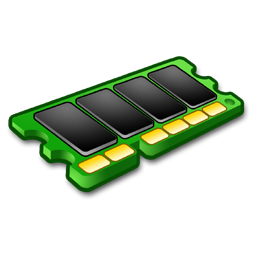
\includegraphics[width=.20\textwidth]{images/cpu-mem.png}};

    \node[inner sep=0pt, right=of cpu-mem] (gpu-mem)
    {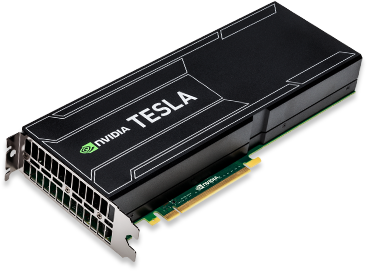
\includegraphics[width=.20\textwidth]{images/gpu-card.png}};

    \draw[*->] let \p1 = (block-5-2.one), \p2 = (block-5-2.center) in (\x1,\y2)    -- (CPU_device);
    \draw[*->] let \p1 = (block-5-2.second), \p2 = (block-5-2.center) in (\x1,\y2) -- (GPU_device);

    \draw[*->] (CPU_device-6-2.center) -- (cpu-mem);
    \draw[*->] (GPU_device-6-2.center) -- (gpu-mem);
  \end{tikzpicture}
  \caption{\texttt{Block} and \texttt{Device\_Info} structure}\label{fig:Device\_Info Structure}
\end{figure}

Using the meta data and specifically \texttt{data\_version\_}, the runtime can keep
track of changes in data on different devices and find the device with latest
data by comparing version numbers:

\begin{algorithm} {Block::get\_latest\_device() $\rightarrow$ Device\_Info}
  \singlespacing

  \begin{algorithmic}[1]
    \Function{Block::get\_latest\_device}{}
    \State $highest\_version\_found \gets 0$
    \State $highest\_version\_device \gets null$
    \ForAll{$device\_info\ in\ this->devices$}
    \If{$device\_info.data\_version > highest\_version\_found$}
    \State {$highest\_version\_found \gets info.data\_version$}
    \State {$highest\_version\_device \gets device\_info$}
    \EndIf
    \EndFor
    \State \Return $highest\_version\_device$
    \EndFunction
    % \hline
  \end{algorithmic}
\end{algorithm}

After determining the device with latest version of data, the runtime can update
other devices if needed. The only interfacing function exposed outside of
\texttt{Block} class is \texttt{get\_data(deviceid)} which returns pointer to memory
location on device identified by \texttt{deviceid}. The logic to always return
latest version of data can be embedded into \texttt{get\_data(device)}:

\begin{algorithm}  {Block::get\_data(deviceid) $\rightarrow$ double*}
  \singlespacing

  \begin{algorithmic}[1]
    \Function{Block::get\_data}{deviceid}
    \State $latest\_device \gets this->get\_latest\_device()$
    \If{$latest\_device.data\_version > this->devices[deviceid]$}
    \State {$memcpy(latest\_device.data,\ this->devices[deviceid].data)$}
    \EndIf
    \State \Return $this->devices[deviceid].data$
    \EndFunction
    % \hline
  \end{algorithmic}
  \label{alg:get_data}
\end{algorithm}

\section{Optimizing Block Transfers}
A enormous cost has to be paid~\cite{Bakkum2010}\cite{memorytransferoverhead}
for transferring memory to GPU as compared to the time taken for actual computation
on GPU. Hence to have significant speed gains by executing on GPU over executing
on CPU, it is necessary to minimize time spent on block transfers. This has been
achieved in by deploying multiple optimizations that are explained in this section.

\subsection{Reducing Block Transfers}
The SIAL runtime has the information about intent of each block request, whether
the block is being requested to be read or written. Using this information the
number of synchronizations between devices can be reduced. The blocks which are
going to be written need not be synchronized, however the blocks requested for
being read or updated need to be synchronized for the requested device.

The algorithm presented in~\ref{alg:get_data} can be split into
\texttt{get\_data} and a explicit \texttt{update\_data}:

\begin{algorithm}  {Block::get\_data(deviceid) $\rightarrow$ double*}
  \singlespacing

  \begin{algorithmic}[1]
    \Function{Block::get\_data}{deviceid}
    \State \Return $this->devices[deviceid].data$
    \EndFunction

    \Function{Block::update\_data}{deviceid}
    \State $latest\_device \gets this->get\_latest\_device()$
    \If{$latest\_device.data\_version > this->devices[deviceid]$}
    \State {$memcpy(latest\_device.data,\ this->devices[deviceid].data)$}
    \EndIf
    \EndFunction
    % \hline
  \end{algorithmic}
\end{algorithm}

This relatively simple change in organization of code along with the information
about intent of the request reduced the synchronizations by TODO\%.

\section{Memory Pinning}
The memory allocated on CPU or main memory is pageable by default. The GPU cannot
access data on such pageable host memory~\cite{datatransferoptimization}
\cite{programmingguidecuda}. For this reason when a memory copy operation is requested
from host to the GPU, the CUDA driver first allocates a temporary \textbf{page locked},
or \textit{pinned} memory on host (main memory) and copies the host memory to the
temporary pinned memory and then finally transfers the memory from pinned memory
to GPU device memory.

- Async Memcpy: eager push

\section{CUDA aware MPI}
- MPI get async % exploiting gpu
\chapter{EXPERIMENTS AND RESULTS}\label{results}

This thesis present a few of the possible performance optimizations on looping
constructs for SIA. These optimizations primarily aimed to reduce the network
operation cost and computing cost. This section describes series of experiments
conducted by varying input parameters such as block size as well as the optimization
parameters such as number of blocks to prefetch and its effects on the performance
of the system.

\section{Environment}
These experiments were carried on HiperGator Computer at UF. Table~\ref{tab:hpg2spec}
describes the specification of HiperGator 2. Table~\ref{tab:hpgcomputespecs}
explains the specifications of HiperGator 2 \textbf{compute} nodes and
table~\ref{tab:hpggpuspecs} explains the specifications of HiperGator 2 \textbf{GPU}
nodes. The table~\ref{tab:hpgconnectspecs} describes the specification for the
node interconnect in HiperGator 2.

\begin{table}[h]
  \centering
  \begin{tabular}{l | c}
    \hline
    Name        & Specifications  \\
    \hline
    Total Cores & 30,000          \\
    Memory      & 120 Terabytes   \\
    Storage     & 1 Petabytes     \\
    Max Speed   & 1,100 Teraflops \\
    \hline
  \end{tabular}
  \caption{HiperGator 2 Spec Sheet}
  \label{tab:hpg2spec}
\end{table}

\begin{table}[h]
  \centering
  \begin{tabular}{l | c}
    \hline
    Name                       & Specification     \\
    \hline
    Manufacturer               & Dell Technologies \\
    Processor                  & Intel E5-2698v3   \\
    Base Processor Frequency   & 2.3 GHz           \\
    Sockets                    & 2                 \\
    Cores per socket           & 16                \\
    Thread(s) per core         & 1                 \\
    Memory per node            & 128 Gigabytes     \\
    Memory Frequency           & 2133 MHz DDR4     \\
    \hline
  \end{tabular}
  \caption{HiperGator 2 \textbf{Compute} Node}
  \label{tab:hpgcomputespecs}
\end{table}

\begin{table}[h]
  \centering
  \begin{tabular}{l | c}
    \hline
    Name                       & Specification     \\
    \hline
    Manufacturer               & Dell Technologies \\
    Processor                  & Intel E5-2683     \\
    Base Processor Frequency   & 2.0 GHz           \\
    Sockets                    & 2                 \\
    Cores per socket           & 14                \\
    Thread(s) per core         & 1                 \\
    GPU                        & Tesla K80         \\
    Memory per node            & 128 Gigabytes     \\
    Memory Frequency           & 2133 MHz DDR4     \\
    \hline
  \end{tabular}
  \caption{HiperGator 2 \textbf{GPU} Node}
  \label{tab:hpggpuspecs}
\end{table}

\begin{table}[h]
  \centering
  \begin{tabular}{l | c}
    \hline
    Name             & Specification                                 \\
    \hline
    Node Connection  & Mellanox 56Gbit/s FDR InfiniBand interconnect \\
    Core Switches    & 100 Gbit/s EDR InfiniBand standard            \\
    \hline
  \end{tabular}
  \caption{HiperGator 2 Node interconnect specification}
  \label{tab:hpgconnectspecs}
\end{table}

\section{Prefetching}
This section presents several experiments conducted to investigate the optimal
parameters and tradeoffs involved in the selection of the parameters.

\subsection{\texttt{hit\_ratio}}
To understand the performance of the prefetching mechanism a new metric is introduced.
Prefetch \texttt{hit\_ratio} is defined as the ratio of the number of times the
SIA runtime did not have to block for a certain data block to be ready and total
number of times the data block is accessed:
\[
  \texttt{hit\_ratio} = \frac{number~of~times~no~blocking~required}{total~number~of~times~data~accessed}
\]
The \texttt{hit\_ratio} represents the number of times prefetching was successful
to hide network transfer cost. In the following experiments \texttt{hit\_ratio}
will be used where appropriate to measure effectiveness of parameters in prefetching.

\subsection{Index Length}
The length of indices is the length of the range of indices involved in the loop.
The length of indices can have high impact on prefetching. To study this relation
between index length and prefetching, \texttt{hit\_ratio} is observed by varying
the range of indices. This is presented in figure~\ref{fig:hitratio}.
\begin{figure}[h]
  \input{results/index_length/hitratio}
  \caption{Index Range Length v/s \texttt{hit\_ratio}}
  \label{fig:hitratio}
\end{figure}

Note that the runtime has to block for data only first time it accesses a block.
Subsequent accesses do not need any blocking since the data is ready. Hence the
\texttt{hit\_ratio} with no prefetching is non zero.

If a index spans only 1 then there is no scope for the runtime to do prefetching.
This is evident from the plot when index length is 1, the \texttt{hit\_ratio} with
prefetching is equal to with no prefetching. As range of index length increased,
prefetching gets working. This can be easily observed from exponential growth in
\texttt{hit\_ratio}. And eventually the curve for \texttt{hit\_ratio} flattens out
after 6 since no significant improvement is achieved by increasing the index range
length.

It is observed that as the runtime requests for multiple blocks for prefetching,
the first request to server takes longer as number of index range increases. This
side effect can be explained using the preceding observation about \texttt{hit\_ratio}.
Since the increase in index range length activates prefetching the first request
to server becomes costlier. This is presented in figure~\ref{fig:p_first_mean}.
\begin{figure}[h]
  \input{results/index_length/p_first_mean}
  \caption{Index Range v/s \texttt{wait\_time\_} per iteration}
  \label{fig:p_first_mean}
\end{figure}

It can be concluded from previous observation that prefetching increases the time
for the first request to server. Thus to compensate for the high cost of first
iteration by offsetting it in subsequent iterations the length of index range to
should be sufficient enough. The mean time taken per iteration is plotted against
the length of index range in figure~\ref{fig:p_np_mean}.

\begin{figure}[h]
  \input{results/index_length/p_np_mean}
  \caption{Index Range v/s \texttt{wait\_time\_} per iteration in Prefetched and no Prefetched Loop}
  \label{fig:p_np_mean}
\end{figure}

The length of index should be around 5 to decrease the \texttt{wait\_time\_}
by factor of 2. The mean \texttt{wait\_time} per iteration with prefetching can
reduce upto 3 times as compared to with no prefetching if the length of index
length is greater than 9.

\subsection{Block Size}
Since the time to transfer block over network is related to size of the block, the
block size affects the first request made during prefetching. Along with the first
request, multiple requests for prefetching subsequent blocks are made. This makes
the \texttt{wait\_time\_} for first call sensitive to block size. This is evident
from the graph plotting Block Size against mean \texttt{wait\_time} for first
iteration in figure~\ref{fig:first_wait_time}.
\begin{figure}[h]
  \input{results/block_size/first_wait_time}
  \caption{Block Size v/s \texttt{wait\_time\_} for first iteration}
  \label{fig:first_wait_time}
\end{figure}

As the block size increases, \texttt{wait\_time\_} for first iteration for loops
with prefetch grows much faster than loops without prefetch. At block of size
greater than 500 elements \texttt{wait\_time\_} for first iteration with prefetch
is almost twice the corresponding \texttt{wait\_time\_} without prefetch.

But once the first request for blocks is made, subsequent iterations are not affected
by the block size as compared to loops in which prefetching is not done, since the
runtime need not block for subsequent blocks. This results in overall reduction
in mean \texttt{wait\_time\_}. This trend is presented in figure~\ref{fig:block_size_avg_wait_time}.
\begin{figure}[h]
  \input{results/block_size/avg_wait_time}
  \caption{Block Size v/s Mean \texttt{wait\_time\_} for Prefetched and No Prefetch Loop}
  \label{fig:block_size_avg_wait_time}
\end{figure}

The mean \texttt{wait\_time\_} grows much slower for loops with prefetch compared
to loops without prefetch.

All of these trends of block size against first and mean \texttt{wait\_time\_} for
loops with and without prefetch are summarized in figure~\ref{fig:block_size_avg_all}
\begin{figure}[h]
  \input{results/block_size/avg_all}
  \caption{Block Size v/s Mean \texttt{wait\_time\_} for Prefetched and No Prefetch Loop}
  \label{fig:block_size_avg_all}
\end{figure}

Although the \texttt{wait\_time\_} for first iteration grows at the highest rate,
prefetching compensates for it and keeps the mean \texttt{wait\_time\_} lower than
without prefetching subsequent blocks.

\subsection{Number of Blocks to Prefetch}
As stated in previous sections, prefetching affects the first request to server
and the size of the block also affects the first request. To observe effect of
number of blocks to prefetch on the initial request, the number of blocks were
varied and plotted against mean \texttt{wait\_time\_} for first request. This is
presented in figure~\ref{fig:look_ahead_first_wait_time}.
\begin{figure}[h]
  \input{results/look_ahead/first_wait_time}
  \caption{Number of Block Prefetched v/s \texttt{wait\_time\_} for first request}
  \label{fig:look_ahead_first_wait_time}
\end{figure}

It is clear from the plot that the mean \texttt{wait\_time\_} for the first request
grows linearly with the number of blocks to prefetch. Thus the number of blocks
to prefetch cannot be set at very high number unless the length of index range is
known to be large.

To determine the effect of number of block to prefetch to prefetching, the number
of blocks to prefetch was varied and is plotted against the mean \texttt{wait\_time\_}.
This plot is presented in figure~\ref{fig:look_ahead_avg_wait_time}.
\begin{figure}[h]
  \input{results/look_ahead/avg_wait_time}
  \caption{Number of Block Prefetched v/s mean \texttt{wait\_time\_}}
  \label{fig:look_ahead_avg_wait_time}
\end{figure}

For the case when the number of block prefetched is 0, which is in the case of no
prefetching the mean \texttt{wait\_time\_} is highest. It drops sharply as the
number of blocks to prefetch increases and then it grows again as increase in number
of blocks to prefetch increases the \texttt{wait\_time\_} for first request to
server.

As the number of blocks to prefetched is increased, more blocks are available for
runtime without blocking. This is presented in figure~\ref{fig:look_ahead_hit_ratio}
by plotting number of blocks to prefetch against \texttt{hit\_ratio}.

\begin{figure}[h]
  \input{results/look_ahead/hit_ratio}
  \caption{Number of Block Prefetched v/s Hit Ratio for first request}
  \label{fig:look_ahead_hit_ratio}
\end{figure}

Hit ratio saturates after hitting a critical amount. There is no much use after
that to increase number of blocks to prefetch. This explains the rise in mean
\texttt{wait\_time\_} as \texttt{wait\_time\_} for first request grows but the
number of blocks available without blocking stays constant.

\section{GPU}
\subsection{Memory Pinning}
\subsubsection{Copy Speed}
\begin{figure}[h]
  \input{results/mempin/block_copy/pin_vs_nopin}
  \caption{Time taken to transfer block to GPU for \textit{pinned} and \textit{non pinned} blocks}
\end{figure}
\subsection{Optimized Transfer}
\begin{figure}[h]
  \input{results/optimized_block_transfer/rccsd_rhf}
  \caption{Optimized v/s Unoptimized Block Tranfers for \texttt{rccsd\_rhf.sialx}}
\end{figure}

\subsection{Memory Pinning Overhead}
\subsubsection{\texttt{alloc}}
\begin{figure}[h]
  \input{results/mempin/overhead/alloc}
  \caption{Pinned and non Pinned memory allocation}
\end{figure}

\subsubsection{\texttt{free}}
\begin{figure}[h]
  \input{results/mempin/overhead/free}
  \caption{Pinned and non Pinned memory de-allocation}
\end{figure} % experiment and result
\chapter{CONCLUSION AND FUTURE WORK}\label{conclusion}
Two approaches to enhance the looping constructs and improve the runtime efficiency
of SIAL interpreter is presented in this thesis. One applies an old technique of
prefetching to data blocks in Super Instruction Architecture. Other improves
the utilization of GPU to execute Super Instructions on GPU and make way to support
other compute devices in future.

Though prefetching makes subsequent requests to a server efficient by reducing or
eliminating \texttt{wait\_time}, it makes the first request to the server expensive.
Thus to make up for it, the length of the range of indices should be long enough. Hit
ratio, as defined in section~\ref{sec:hit_ratio}, can be used as a metric to evaluate
the performance of prefetching. As seen in section~\ref{sec:bp_molecule}, prefetching
helps in reducing overall \texttt{wait\_time} when most of the \texttt{wait\_time}
is due to blocking for data block transfer over the network.

Future work includes exploiting the provision to dynamically vary the number of blocks
to prefetch to strike a balance between high cost of the initial request and relatively
cheap subsequent requests.

Executing Super Instructions on GPU can speed up the computation for bigger block
sizes. Transferring blocks between GPU and main memory is expensive but it can be
avoided or reduced by directly collecting to or sending blocks from GPU memory
buffers and reducing the transfers using other techniques. Page locked memory
can improve memory transfer speed by invoking DMA and bypassing CPU. But page locking
memory is expensive as compared to simple dynamically allocated memory. Page locked
memory blocks can be cached and served with high cache hit ratio.

Further improvement in utilization of GPU can be achieved by implementing more
super instructions on GPU and a way to easily port user defined super instructions
to GPU; By exploiting the asynchronous memory synchronization between GPU memory
and main memory by looking ahead for instruction which needs the memory
to be transferred and initiating the asynchronous transfer as soon as data is ready.
And exploring the feasibility of having access to GPU on the servers and implementing
RDMA to transfer memory blocks between workers and servers. Lastly, implementing
an advanced caching mechanism for page locked memory blocks can be worked upon to have
more memory efficient caching mechanism. % conclusion and future work

%-----------------------------------------------------------------------%

% Use the appropriate file depending upon the number of appendices you have


% TODO uncomment below line
%% The Editorial Office Requirements for the Table of Contents cause a significant problem
%in Latex if there is only one Appendix. The Appendix is no longer labeled "A" in the TOC
%but has the word "APPENDIX" placed in front of the title of the Appendix. This can be done
%without issue IF nothing needs to be numbered by LaTeX in the Appendix. Unfortunately, most of the time
%something needs to be numbered in that single Appendix. For this reason we have included the IFTHENELSE switch
%found in this document and at the beginning of AppendixA. We assume that if you have any appendices, that you have more than one. However, you DO only have one appendix DO NOT USE THIS FILE!!!!!!!!!!!!!!!!!!!!!!!
%
% OneSingleAppendix.tex has all the settings needed to adjust for a single appendix
% you will have a major problem with your TOC if you use this file with a single appendix!!!!!

%
% Comment (or delete) all of the \input{AppendixB} commands except those you are using.
%Then open the AppendixA.tex file and continue there.

%you can add/substract individual appendices through by using the /include{appendix'X'}
% and creating/deleting the appropriate files
\appendix %
%\clearpage%

\addtocontents{toc}{\protect\addvspace{10pt}\noindent{APPENDIX} \protect\hfill\par}{}


% % % % % % % If you have a single appendix, you should be using appendix1.tex
% % % % % % % NOT this file

\chapter{THIS IS THE FIRST APPENDIX}

Lorem ipsum dolor sit amet, consectetuer adipiscing elit. Maecenas
eget magna. Aenean et lorem. Ut dignissim neque at nisi. In hac
habitasse platea dictumst. In porta ornare eros. Nunc eu ante. In
non est vehicula tellus cursus suscipit. Proin sed libero. Sed risus
enim, eleifend in, pellentesque ac, nonummy quis, nulla. Phasellus
imperdiet libero nec massa. Ut sapien libero, adipiscing eu,
volutpat porttitor, ultricies eget, nisi. Sed odio. Suspendisse
potenti. Duis dolor augue, viverra id, porta in, dignissim id, nisl.
Vivamus blandit cursus eros. Maecenas sit amet urna sit amet orci
nonummy pharetra.

Praesent cursus nibh et mauris. In aliquam felis sit amet ligula.
Nulla faucibus nisl eget nisl. Aliquam tincidunt. Mauris eget elit
sed massa luctus posuere. Pellentesque suscipit. In odio urna,
semper ut, convallis ut, porta et, nibh. Nulla sodales metus nec
velit posuere gravida. Cras tristique. Etiam urna risus, accumsan
ut, placerat sed, iaculis id, est.

Nullam mi. Pellentesque habitant morbi tristique senectus et netus
et malesuada fames ac turpis egestas. Duis vitae metus in massa
hendrerit rhoncus. Fusce tortor justo, laoreet eu, facilisis at,
gravida et, felis. Donec imperdiet mollis erat. Integer tempus nulla
ac lorem. Fusce porttitor. Aenean quis arcu. Morbi consectetuer, leo
eu mollis elementum, urna massa malesuada risus, euismod tempor
lorem elit ut mauris. Cras elit orci, facilisis ac, mattis iaculis,
cursus ac, augue. Donec eget nisl. Pellentesque fermentum sodales
nibh. Vivamus non risus. Donec est libero, tincidunt sit amet,
pretium vitae, blandit sed, tellus. Nunc diam risus, interdum sed,
laoreet quis, varius ac, turpis. In et purus eget nibh vehicula
rhoncus. Aenean et neque. Praesent nisl nisi, tempus quis, nonummy
ac, auctor a, neque. Suspendisse et metus. Suspendisse non metus eu
mauris auctor sagittis.
 %
\chapter{AN EXAMPLE OF A HALF TITLE PAGE}%
\label{appendixB}

\clearpage %remove this command if your appendix doesn't start with a landscaped page!!!!!
\thispagestyle{plain}
\begin{landscape}
\begin{figure}

  \begin{center}
    \includegraphics[width=6in]{images/LaTeX2e_logo.eps}
    \caption{\LaTeX 2\ensuremath{\epsilon.} logo}\label{biglogo}
  \end{center}
\end{figure}
\end{landscape}


This is how a section should look if the first page is a landscape page.
Lorem ipsum dolor sit amet, consectetuer adipiscing elit. Ut sit
amet nulla. Integer mauris turpis, dapibus ac, auctor non, vehicula
sit amet, magna. Suspendisse eu tellus. Etiam porta. Donec magna.
Donec ut dui. In hac habitasse platea dictumst. Nullam suscipit, mi
at adipiscing commodo, lorem erat scelerisque erat, non pulvinar leo
mi eu metus. Phasellus id felis. Sed quam purus, molestie quis,
ultrices nec, dictum at, magna. Proin viverra viverra ante.

Maecenas sagittis magna quis ligula. Duis vestibulum mi a felis.
Aenean accumsan mattis massa. Nullam lacus sem, consectetuer non,
condimentum sit amet, pharetra ac, odio. Morbi nisi magna, tincidunt
sed, placerat nec, tincidunt id, lectus. Donec ac dui non mauris
vulputate aliquam. Nullam scelerisque congue pede. Integer ipsum.
Vestibulum auctor. Suspendisse eget leo id libero cursus dictum. Sed
malesuada. Aliquam imperdiet. Donec dui metus, porta eu, aliquet
vel, vulputate vitae, lacus.

Nulla quis purus id turpis luctus feugiat. Fusce feugiat. Proin
felis. Morbi elit est, fermentum in, tincidunt vitae, convallis vel,
orci. Vestibulum justo. Suspendisse non nisl. Pellentesque pretium
adipiscing elit. Phasellus fermentum consequat augue. Sed pede nisl,
fermentum vel, vulputate id, sollicitudin sed, ligula. Cras
suscipit, quam et euismod sagittis, nisl felis gravida felis, quis
pulvinar purus est vel pede. Suspendisse mattis est ac nunc.
Curabitur rutrum, turpis sit amet commodo tempus, metus lorem
commodo lectus, eget fringilla justo nisi et purus. Ut quam sapien,
vehicula quis, rhoncus non, sagittis nec, risus.

Donec eget augue ac lacus adipiscing porta. Maecenas pede. Vivamus
molestie. Duis condimentum ligula auctor pede. Nullam ullamcorper
rhoncus erat. Ut ornare interdum urna. Suspendisse potenti.
Curabitur mattis mauris nec risus. Aenean iaculis turpis eu tortor.
Donec nec ante non mauris pellentesque fringilla.

Phasellus vitae dui id orci sodales cursus. Curabitur sed nulla quis
mauris tincidunt iaculis. Vivamus semper semper orci. Phasellus
suscipit ante vitae leo. Sed arcu ipsum, condimentum id, luctus in,
sodales eu, magna. In dictum, arcu quis pharetra vestibulum, ante
enim placerat lacus, vitae placerat est leo vitae elit. Pellentesque
bibendum enim vulputate eros. Nunc laoreet. Pellentesque habitant
morbi tristique senectus et netus et malesuada fames ac turpis
egestas. Praesent purus odio, euismod sit amet, aliquam a, volutpat
in, augue. Phasellus id massa. Suspendisse suscipit ligula pharetra
dolor. Pellentesque vel pede.

Aliquam pharetra est sit amet magna. Aliquam varius. Donec eu lectus
et nisl iaculis porttitor. Morbi mattis, mauris sed luctus
hendrerit, nulla velit molestie dolor, ac volutpat urna augue vel
quam. Maecenas pellentesque libero et massa. Integer vestibulum,
lacus at mattis euismod, nisl arcu commodo lectus, ut euismod dolor
ligula sit amet libero. Nam in ligula sit amet ante eleifend
aliquet. Phasellus feugiat erat at nulla. Proin in lectus. Proin
laoreet leo laoreet leo congue lacinia. Quisque non diam sit amet
enim ultrices commodo. Praesent fermentum lectus sed ligula. Integer
pulvinar accumsan pede. Quisque molestie ligula eget odio.
Vestibulum ante ipsum primis in faucibus orci luctus et ultrices
posuere cubilia Curae;
 %
\chapter{DERIVATION OF THE $\Upsilon$ FUNCTION}%
\label{appendixC}

%\clearpage %remove this command if your appendix doesn't start with a landscaped page!!!!!
%\thispagestyle{plain}
%\begin{landscape}
%\begin{figure}

 % \begin{center}
  %  \includegraphics[width=6in]{LaTeX2e_logo.eps}
   % \caption{\LaTeX 2\ensuremath{\epsilon.} logo}\label{biglogo}
  %\end{center}
%\end{figure}
%\end{landscape}

%%%%%%%%%%%%%%%%%%%%%%%%%%%%%%%%%%%%%%%%%%%%%%%%%%%%%%%%%%%%%%%%%%%%%%%%%%%%%%%%%%%%%%%%%%%%%%%%%%


%ADD LABEL

%%%%%%%%%%%%%%%%%%%%%%%%%%%%%%%%%%%%%%%%%%%%%%%%%%%%%%%%%%%%%%%%%%%%%%%%%%%%%%%%%%%%%%%%%%%%%%%%%%

\proposition{The Upsilon Function}

(1) If $\beta>0$ and $\alpha\neq0$, then for all $n\geq-1$,

$$I_{n}(c;\alpha; \beta; \delta) = - \frac{e^{\alpha c}}{\alpha} \sum_{i=0}^{n}(\frac{\beta}{\alpha})^{n-i} Hh_{i}(\beta c -\delta)$$

$$+ (\frac{\beta}{\alpha})^{n+1} \frac{\sqrt{2 \pi}}{\beta} e^{\frac{\alpha \delta}{\beta}+\frac{\alpha^{2}}{2\beta^{2}}} \phi(-\beta c + \delta + \frac{\alpha}{\beta})$$
(2) If $\beta<0$ and $\alpha<0$, then for all $x \geq -1$

$$I_{n}(c;\alpha; \beta; \delta) = - \frac{e^{\alpha c}}{\alpha} \sum_{i=0}^{n}(\frac{\beta}{\alpha})^{n-i} Hh_{i}(\beta c -\delta)$$

$$- (\frac{\beta}{\alpha})^{n+1} \frac{\sqrt{2 \pi}}{\beta} e^{\frac{\alpha \delta}{\beta}+\frac{\alpha^{2}}{2\beta^{2}}} \phi(\beta c - \delta - \frac{\alpha}{\beta})$$

\begin{proof}{Case 1.}

$\beta>0$ and $\alpha\neq0$. Since, for any constant $\alpha$ and $n \geq 0$, $e^{\alpha x} Hh_{n}(\beta x - \delta) \rightarrow 0$ as $x \rightarrow \infty$ thanks to (B4), integration by parts leads to

$$I_{n}=-\frac{1}{\alpha}Hh(\beta c -\delta) e^{\alpha c} + \frac{\beta}{\alpha}\int_{c}^{\infty} e^{\alpha x} Hh_{n-1}(\beta c - \delta)dx$$

In other words, we have a recursion, for $n \geq 0$, $I_{n}=-(e^{\alpha c}{\alpha})Hh_{n}(\beta c - \delta) + (\frac{\beta}{\alpha})I_{n-1}$ with

$$I_{-1}=\sqrt{2 \pi} \int_{c}{\infty}e^{\alpha x}\varphi(-\beta x +\delta)dx$$

$$=\frac{\sqrt{2 \pi}}{\beta} e^{\frac{\alpha \delta}{\beta}+\frac{\alpha^{2}}{2 \beta^{2}}}\phi(-\beta c + \delta +\frac{\alpha}{\beta})$$

Solving it yields, for $n \geq -1$,

$$I_{n}=-\frac{e^{\alpha c}}{\alpha}\sum_{i=0}^{n}(\frac{\beta}{\alpha})^{i}Hh_{n-i}(\beta c+\delta) + (\frac{\beta}{\alpha})^{n+1}I_{-1}$$

$$=-\frac{e^{\alpha c}}{\alpha}\sum_{i=0}^{n}(\frac{\beta}{\alpha})^{n-i} Hh_{i}(\beta c+\delta)$$

$$+ (\frac{\beta}{\alpha})^{n+1}\frac{\sqrt{2 \pi}}{\beta} e^{\frac{\alpha \delta}{\beta}+\frac{\alpha^{2}}{2 \beta^{2}}}\phi(-\beta c + \delta +\frac{\alpha}{\beta})$$

where the sum over an empty set is defined to be zero.
\end{proof}

Case2. $\beta<0$ and $\alpha<0$. In this case, we must also have, for $n \geq 0$ and any constant $\alpha<0, e^{\alpha x}Hh_{n}(\beta x -\delta) \rightarrow 0$ as

$x \rightarrow \infty$, thanks to (B5). Using integration by parts, we again have the same recursion, for $n \geq 0, I_{n}=-(e^{\alpha c}/\alpha)Hh_{n}(\beta c - \delta)+(\beta / \alpha)I_{n-1}$, but with a different initial condition

$$I_{-1}=\sqrt{2 \pi}\int_{c}^{\infty}e^{\alpha x}\varphi(-\beta x + \delta)dx$$

$$=-\frac{\sqrt{2 \pi}}{\beta} exp\{\frac{\alpha \delta}{\beta}+\frac{\alpha^{2}}{2 \beta^{2}}\}\phi(\beta c - \delta -\frac{\alpha}{\beta})$$

Solving it yields (B8), for $n \geq -1$.

Finally, we sum the double exponential and the normal random variables

Proposition B.3.

Suppose $\{\xi_{1},\xi_{2},...\}$ is a sequence of i.i.d. exponential random variables with rate $\eta>0$, and Z is a normal variable with distribution $N(0,\sigma^{2})$. Then for every $ n \geq 1$, we have: (1) The density functions are given by:

$$f_{Z+\sum_{i=1}^{n}\xi_{i}}(t)=(\sigma\eta)^{n}\frac{e^{(\sigma\eta)^{2}/2}}{\sigma\sqrt{2\pi}}e^{-t\eta}Hh_{n-1}(-\frac{t}{\sigma}+\sigma\eta)$$

$$f_{Z-\sum_{i=1}^{n}\xi_{i}}(t)=(\sigma\eta)^{n}\frac{e^{(\sigma\eta)^{2}/2}}{\sigma\sqrt{2\pi}}e^{-t\eta}Hh_{n-1}(\frac{t}{\sigma}+\sigma\eta)$$
(2) The tail probabilities are given by

$$P(Z+\sum_{i=1}^{n}\xi_{i}\geq x) = (\sigma\eta)^{n}\frac{e^{(\sigma\eta)^{2}/2}}{\sigma\sqrt{2\pi}}e^{-t\eta}I_{n-1}(x;-\eta,-\frac{1}{\sigma},-\sigma\eta)$$

$$P(Z-\sum_{i=1}^{n}\xi_{i}\geq x) = (\sigma\eta)^{n}\frac{e^{(\sigma\eta)^{2}/2}}{\sigma\sqrt{2\pi}}e^{-t\eta}I_{n-1}(x;\eta,\frac{1}{\sigma},-\sigma\eta)$$

Proof. Case 1. The densities of $Z+\sum_{i=1}^{n}\xi_{i}$, and $Z-\sum_{i=1}^{n}\xi_{i}$. We have

$$f_{Z+\sum_{i=1}^{n}\xi_{i}}(t)=\int_{-\infty}^{\infty}f_{\sum_{i=1}^{n}\xi_{i}}(t-x)f_{Z}(x)dx$$

$$=e^{-t\eta}(\eta^{n})\int_{-\infty}{t}\frac{e^{x\eta}(t-x)^{n-1}}{(n-1)!}\frac{1}{\sigma\sqrt{2\pi}}e^{-x^{2}/(2\sigma^{2})}dx$$

$$=e^{-t\eta}(\eta^{n})e^{(\sigma\eta)^{2}/(2)}\int_{-\infty}{t}\frac{(t-x)^{n-1}}{(n-1)!}\frac{1}{\sigma\sqrt{2\pi}}e^{-(x-\sigma^{2}\eta)^{2}/(2\sigma^{2})}dx$$

Letting $y=(x-\sigma^{2}\eta)/\sigma$ yields

$$f_{Z+\sum_{i=1}^{n}\xi_{i}}(t)=e^{-t\eta}(\eta^{n})e^{(\sigma\eta)^{2}/(2)}\sigma^{n-1}$$

$$\times\int_{-\infty}^{t/\sigma-\sigma\eta}\frac{(t/\sigma - y -\sigma\eta)^{n-1}}{(n-1)!}\frac{1}{\sqrt{2\pi}}e^{-y^{2}/2}dy$$

$$=\frac{e^{(\sigma\eta)^{2}/2}}{\sqrt{2\pi}}(\sigma^{n-1}\eta^{n})e^{-t\eta}Hh_{n-1}(-t/\sigma + \sigma\eta)$$

because $(1/(n-1)!)\int_{-\infty}{a}(a-y)^{n-1}e^{-y^{2}/2}dy=Hh_{n-1}(a)$. The derivation of $f_{Z+\sum_{i=1}^{n}\xi_{i}}(t)$ is similar.

Case 2. $P(Z+\sum_{i=1}^{n}\xi_{i}\geq x)$ and $P(Z-\sum_{i=1}^{n}\xi_{i}\geq x)$. From (B9), it is clear that

$$P(Z+\sum_{i=1}^{n}\xi_{i}\geq x)=\frac{(\sigma\eta)^{n}e^{(\sigma\eta)^{2}/2}}{\sigma\sqrt{2\pi}}\int_{x}^{\infty}e^{(-i\eta)}Hh_{n-1}(-\frac{t}{\sigma}+\sigma\eta)dt$$

$$=\frac{(\sigma\eta)^{n}e^{(\sigma\eta)^{2}/2}}{\sigma\sqrt{2\pi}}I_{n-1}(x;-\eta,-\frac{1}{\sigma},-\sigma\eta)dt$$

by (B6). We can compute
$P(Z-\sum_{i=1}^{n}\xi_{i}\geq x)$ similarly.

\theorem{Theorem} With $\pi_{n}:= P(N(t)=n)=e^{-\lambda T}(\lambda T)^{n}/n!$ and $I_{n}$ in Proposition \ref{first}.
, we have

$$P(Z(T)\geq a)=\frac{e^{(\sigma \eta_{1})^{2} T/2}}{\sigma \sqrt{2 \pi T}} \sum_{n=1}^{\infty} \pi_{n} \sum_{k=1}^{n} P_{n,k}(\sigma\sqrt{T}\eta_{1})^{k}\times I_{k-1}(a-\mu T; -\eta_{1},-\frac{1}{\sigma\sqrt{T}},-\sigma\eta_{1}\sqrt{T})$$

$$+\frac{e^{(\sigma\eta_{2})^{2}T/2}}{\sigma\sqrt{2\pi T}}\sum_{n=1}^{\infty}\pi_{n}\sum_{k=1}^{n}Q_{n,k}(\sigma\sqrt{T}\eta_{2})^{k}$$

$$\times I_{k-1}(a-\mu T; \eta_{2},\frac{1}{\sigma\sqrt{T}},-\sigma\eta_{2}\sqrt{T})$$

$$+\pi_{0}\phi(-\frac{a-\mu T}{\sigma\sqrt{T}})$$

Proof by the decomposition (B2)

$$P(Z(T) \geq a)= \sum_{n=0}^{\infty}\pi_{n} P(\mu T +\sigma\sqrt{T} Z + \sum_{j=1}^{n}Y_{j} \geq a)$$

$$=\pi_{0}P(\mu T +\sigma\sqrt{T} Z  \geq a)$$

$$+\sum_{n=1}^{\infty}\pi_{n}\sum_{k=1}^{n}P_{n,k} P(\mu T +\sigma\sqrt{T} Z + \sum_{j=1}^{n}\xi_{j}^{+} \geq a)$$

$$+\sum_{n=1}^{\infty}\pi_{n}\sum_{k=1}^{n}Q_{n,k} P(\mu T +\sigma\sqrt{T} Z - \sum_{j=1}^{n}\xi_{j}^{-} \geq a)$$

The result now follows via (B11) and (B12) for $\eta_{1} > 1$ and $\eta_{2} >0$.


 %
\chapter{DERIVATION OF THE $\Upsilon$ FUNCTION}%
\label{appendixB}

%\clearpage %remove this command if your appendix doesn't start with a landscaped page!!!!!
%\thispagestyle{plain}
%\begin{landscape}
%\begin{figure}

% \begin{center}
  %  \includegraphics[width=6in]{LaTeX2e_logo.eps}
   % \caption{\LaTeX 2\ensuremath{\epsilon.} logo}\label{biglogo}
  %\end{center}
%\end{figure}
%\end{landscape}

%%%%%%%%%%%%%%%%%%%%%%%%%%%%%%%%%%%%%%%%%%%%%%%%%%%%%%%%%%%%%%%%%%%%%%%%%%%%%%%%%%%%%%%%%%%%%%%%%%

%ADD LABEL

%%%%%%%%%%%%%%%%%%%%%%%%%%%%%%%%%%%%%%%%%%%%%%%%%%%%%%%%%%%%%%%%%%%%%%%%%%%%%%%%%%%%%%%%%%%%%%%%%%

We first decompose the sum of the double exponential random variables.

The memoryless property of exponential random variables yields $(\xi^{+}-\xi^{-}|\xi^{+}>\xi^{-})=^{d}\xi^{+}$ and $(\xi^{+}-\xi^{-}|\xi^{+}<\xi^{-})=^{d}-\xi^{-}$, thus leading to the conclusion that

\begin{equation*}
\xi^{+}-\xi^{-} =\left\{
\begin{array}{rl}
\xi^{+} & \text{with probability $\eta_{2}/(\eta_{1}+\eta_{2})$ }\\
-\xi^{-} & \text{with probability $\eta_{1}/(\eta_{1}+\eta_{2})$ }
\end{array}\right\}.
\end{equation*}

because the probabilities of the events $\xi^{+}>\xi^{-}$ and $\xi^{+}<\xi^{-}$ are $\eta_{2}/(\eta_{1}+\eta_{2})$ and $\eta_{1}/(\eta_{1}+\eta_{2})$, respectively. The following proposition extends (B.1.)

Proposition B.1. For every $n\geq1$, we have the following decomposition

\begin{equation*}
\sum_{i=1}^{n}Y_{i}=^{d}\left\{
\begin{array}{rl}
\sum_{i=1}^{k}\xi_{i}^{+} & \text{with probability $P_{n,k},k=1,2,...,n$ }\\
-\sum_{i=1}^{k}\xi_{i}^{-} & \text{with probability $Q_{n,k},k=1,2,...,n$ }
\end{array}\right\}.
\end{equation*}

where $P_{n,k}$ and $Q_{n,k}$ are given by

$$P_{n,k}=\sum_{i=k}^{n-1}\binom {n-k-1} {i-k}\binom {n} {i}(\frac{\eta_{1}}{\eta_{1}+\eta_{2}})^{i-k}(\frac{\eta_{2}}{\eta_{1}+\eta_{2}})^{n-i}p^{i}q^{n-i}$$

$$1\leq k\leq n-1$$

$$Q_{n,k}=\sum_{i=k}^{n-1}\binom {n-k-1} {i-k}\binom {n} {i}(\frac{\eta_{1}}{\eta_{1}+\eta_{2}})^{n-i}(\frac{\eta_{2}}{\eta_{1}+\eta_{2}})^{i-k}p^{n-i}q^{i}$$

$$1\leq k\leq n-1, P_{n,n}=p^{n},Q_{n,n}=q^{n}$$

and $\binom{0}{0}$ is defined to be one. Hence $\xi_{i}^{+}$ and $\xi_{i}^{-}$ are i.i.d. exponential random variables with rates $\eta_{1}$ and $\eta_{2}$, respectively.

As a key step in deriving closed-form solutions for call and put options, this proposition indicates that the sum of the i.i.d. double exponential random variable can be written, in distribution, as a randomly mixed gamma random variable. To prove Proposition B.1, the following lemma is needed.

Lemma B.1.

$$\sum_{i=1}^{n}\xi_{i}^{+}-\sum_{i=1}^{n}\xi_{i}^{-}$$

\begin{equation*}
=^{d}\left\{
\begin{array}{rl}
\sum_{i=1}^{k}\xi_{i} & \text{with probability $\binom {n-k+m-1} {m-1}(\frac{\eta_{1}}{\eta_{1}+\eta_{2}})^{n-k}(\frac{\eta_{2}}{\eta_{1}+\eta_{2}})^{m}, k=1,...,n$ }\\
-\sum_{i=1}^{l}\xi_{i} & \text{with probability $\binom {n-l+m-1} {n-1}(\frac{\eta_{1}}{\eta_{1}+\eta_{2}})^{n}(\frac{\eta_{2}}{\eta_{1}+\eta_{2}})^{m-l}, l=1,...,m$ }
\end{array}\right\}.
\end{equation*}

We prove it by introducing the random variables $A(n,m) = \sum_{i=1}^{n}\xi_{i}-sum_{j=1}^{m}\tilde{\xi}_{j}$ Then

\begin{equation*}
A(n,m) =^{d}\left\{
\begin{array}{rl}
A(n-1,m-1)+\xi^{+} & \text{with probability $\eta_{2}/(\eta_{1}+\eta_{2})$ }\\
A(n-1,m-1)-\xi^{-} & \text{with probability $\eta_{1}/(\eta_{1}+\eta_{2})$ }
\end{array}\right\}.
\end{equation*}

\begin{equation*}
 =^{d}\left\{
\begin{array}{rl}
A(n,m-1) & \text{with probability $\eta_{2}/(\eta_{1}+\eta_{2})$ }\\
A(n-1,m) & \text{with probability $\eta_{1}/(\eta_{1}+\eta_{2})$ }
\end{array}\right\}.
\end{equation*}

via B.1.. Now suppose horizontal axis that are representing the number of $\{\zeta_{i}^{+}\}$ and vertical axis representing the number of $\{\zeta_{i}^{-}\}$. Suppose we have a random walk on the integer lattice points. Starting from any point $(n,m),n,m \geq 1$, the random walk goes either one step to the left with probability $\eta_{1}/(\eta_{1}+\eta_{2})$ or one step down with probability $\eta_{2}/(\eta_{1}+\eta_{2})$, and the random walks stops once it reaches the horizontal or vertical axis. For any path from (n,m) to (k,0) , $1 \geq k \geq n$, it must reach (k,1) first before it makes a final move to (k,0). Furthermore, all the paths going from (n,m) to (k,1) must have exactly n-k lefts and m-1 downs, whence the total number of such paths is $\binom {n-k+m-1}{m-1}$. Similarly the total number of paths from (n,m) to (0,l) , $1 \geq l \geq m$, is $\binom {n-l+m-1}{n-1}$. Thus

\begin{equation*}
A(n,m)=^{d}\left\{
\begin{array}{rl}
\sum_{i=1}^{k}\xi_{i} & \text{with probability $\binom {n-k+m-1} {m-1}(\frac{\eta_{1}}{\eta_{1}+\eta_{2}})^{n-k}(\frac{\eta_{2}}{\eta_{1}+\eta_{2}})^{m}, k=1,...,n$ }\\
-\sum_{i=1}^{l}\xi_{i} & \text{with probability $\binom {n-l+m-1} {n-1}(\frac{\eta_{1}}{\eta_{1}+\eta_{2}})^{n}(\frac{\eta_{2}}{\eta_{1}+\eta_{2}})^{m-l}, l=1,...,m$ }
\end{array}\right\}.
\end{equation*}

and the lemma is proven.

Now, let's prove the proposition B.1. By the same analogy used in Lemma B.1 to compute probability $P_{n,m},1\geq k \geq n$, the probability weight assigned to $\sum_{i=1}^{k}\xi_{i}^{+}$ when we decompose $\sum_{i=1}^{k}Y_{i}$, it is equivalent to consider the probability of the random walk ever reach (k,0) starting from the point (i,n-i) being $\binom {n}{i}p^{i}q^{n-i}$. Note that the point (k,0) can only be reached from point (i,n-i) such that $k \geq i \geq n-1$, because the random walk can only go left or down, and stops once it reaches the horizontal axis. Therefore, for $1 \geq k \geq n-1$, (B3) leads to

$$P_{n,k}=\sum_{i=k}{n-1}P(going from (i,n-i) to (k,0)). P(starting from (i,n-i))$$

$$=\sum_{i=k}^{n-1}\binom {i+(n-i)-k-1} {(n-i)-1}\binom {n} {i}(\frac{\eta_{1}}{\eta_{1}+\eta_{2}})^{i-k}(\frac{\eta_{2}}{\eta_{1}+\eta_{2}})^{n-i}p^{i}q^{n-i}$$

$$=\sum_{i=k}^{n-1}\binom {n-k-1} {n-i-1}\binom {n} {i}(\frac{\eta_{1}}{\eta_{1}+\eta_{2}})^{i-k}(\frac{\eta_{2}}{\eta_{1}+\eta_{2}})^{n-i}p^{i}q^{n-i}$$

$$=\sum_{i=k}^{n-1}\binom {n-k-1} {i-k}\binom {n} {i}(\frac{\eta_{1}}{\eta_{1}+\eta_{2}})^{i-k}(\frac{\eta_{2}}{\eta_{1}+\eta_{2}})^{n-i}p^{i}q^{n-i}$$

Of course $P_{n,n}=p^{n}$. Similarly, we can compute $Q_{n,k}$:

$$Q_{n,k}=\sum_{i=k}{n-1}P(going from (n-i,i) to (0,k)). P(starting from (n-i,i))$$

$$=\sum_{i=k}^{n-1}\binom {i+(n-i)-k-1} {(n-i)-1}\binom {n} {n-i}(\frac{\eta_{1}}{\eta_{1}+\eta_{2}})^{n-i}(\frac{\eta_{2}}{\eta_{1}+\eta_{2}})^{i-k}p^{n-i}q^{i}$$

$$=\sum_{i=k}^{n-1}\binom {n-k-1} {i-k}\binom {n} {i}(\frac{\eta_{1}}{\eta_{1}+\eta_{2}})^{n-i}(\frac{\eta_{2}}{\eta_{1}+\eta_{2}})^{i-k}p^{n-i}q^{i}$$

with $Q_{n,n}=q^{n}$. Incidentally, we have also got $\sum{k=1}{n}(P_{n,k}+Q_{n,k})=1$

B.2. Let's develop now the results on Hh functions.
First of all, note that $Hh_{n}(x)\rightarrow 0$, as $x \rightarrow \infty$, for $n \geq -1$; and $Hh_{n}(x) \rightarrow \infty$, as $x \rightarrow -\infty$, for $n \geq -1$; and $Hh_{0}(x)=\sqrt{2\pi} \phi(-x) \rightarrow \sqrt{2\pi}$, as $x \rightarrow -\infty$. Also, for every $n \geq -1$, as $x \rightarrow \infty$,

$$lim Hh_{n}(x)/\{\frac{1}{x^{n+1}}e^{-\frac{x^{2}}{2}}\}=1$$

and as $x \rightarrow \infty$

$$Hh_{n}(x)=O(|x|^{n})$$

Here (B4) is clearly true for $n=-1$, while for $n \geq 0$ note that as $x\rightarrow _\infty$,

$$Hh_{n}(x)=\frac{1}{n!}\int_{x}{\infty}(t-x)^{n}e^{-\frac{t^{2}}{2}}dt$$

$$\leq \frac{2^{n}}{n!}\int_{-\infty}^{\infty}|t|^{n}e^{-t^{2}}{2}dt+\frac{2^{n}}{n!}\int{-\infty}{\infty}|x|^{n}e^{-t^{2}}{2}dt=O(|x|^{n})$$

For option pricing it is important to evaluate the integral $I_{n}(c;\alpha;\beta;\delta)$,

$$I_{n}(c;\alpha;\beta;\delta)=\int_{c}{\infty}e^{\alpha x}Hh_{n}(\beta x-\delta)dx, n\geq 0$$

for arbitrary constants $\alpha, c$ and $\beta$.
 %
%\input{tex/appendixE} % %These files aren't included in the template
%\input{tex/appendixF} %
%\chapter{DERIVATION OF THE $\Upsilon$ FUNCTION}%
\label{appendixC}

%\clearpage %remove this command if your appendix doesn't start with a landscaped page!!!!!
%\thispagestyle{plain}
%\begin{landscape}
%\begin{figure}

 % \begin{center}
  %  \includegraphics[width=6in]{LaTeX2e_logo.eps}
   % \caption{\LaTeX 2\ensuremath{\epsilon.} logo}\label{biglogo}
  %\end{center}
%\end{figure}
%\end{landscape}

%%%%%%%%%%%%%%%%%%%%%%%%%%%%%%%%%%%%%%%%%%%%%%%%%%%%%%%%%%%%%%%%%%%%%%%%%%%%%%%%%%%%%%%%%%%%%%%%%%


%ADD LABEL

%%%%%%%%%%%%%%%%%%%%%%%%%%%%%%%%%%%%%%%%%%%%%%%%%%%%%%%%%%%%%%%%%%%%%%%%%%%%%%%%%%%%%%%%%%%%%%%%%%

\proposition{The Upsilon Function}

(1) If $\beta>0$ and $\alpha\neq0$, then for all $n\geq-1$,

$$I_{n}(c;\alpha; \beta; \delta) = - \frac{e^{\alpha c}}{\alpha} \sum_{i=0}^{n}(\frac{\beta}{\alpha})^{n-i} Hh_{i}(\beta c -\delta)$$

$$+ (\frac{\beta}{\alpha})^{n+1} \frac{\sqrt{2 \pi}}{\beta} e^{\frac{\alpha \delta}{\beta}+\frac{\alpha^{2}}{2\beta^{2}}} \phi(-\beta c + \delta + \frac{\alpha}{\beta})$$
(2) If $\beta<0$ and $\alpha<0$, then for all $x \geq -1$

$$I_{n}(c;\alpha; \beta; \delta) = - \frac{e^{\alpha c}}{\alpha} \sum_{i=0}^{n}(\frac{\beta}{\alpha})^{n-i} Hh_{i}(\beta c -\delta)$$

$$- (\frac{\beta}{\alpha})^{n+1} \frac{\sqrt{2 \pi}}{\beta} e^{\frac{\alpha \delta}{\beta}+\frac{\alpha^{2}}{2\beta^{2}}} \phi(\beta c - \delta - \frac{\alpha}{\beta})$$

\begin{proof}{Case 1.}

$\beta>0$ and $\alpha\neq0$. Since, for any constant $\alpha$ and $n \geq 0$, $e^{\alpha x} Hh_{n}(\beta x - \delta) \rightarrow 0$ as $x \rightarrow \infty$ thanks to (B4), integration by parts leads to

$$I_{n}=-\frac{1}{\alpha}Hh(\beta c -\delta) e^{\alpha c} + \frac{\beta}{\alpha}\int_{c}^{\infty} e^{\alpha x} Hh_{n-1}(\beta c - \delta)dx$$

In other words, we have a recursion, for $n \geq 0$, $I_{n}=-(e^{\alpha c}{\alpha})Hh_{n}(\beta c - \delta) + (\frac{\beta}{\alpha})I_{n-1}$ with

$$I_{-1}=\sqrt{2 \pi} \int_{c}{\infty}e^{\alpha x}\varphi(-\beta x +\delta)dx$$

$$=\frac{\sqrt{2 \pi}}{\beta} e^{\frac{\alpha \delta}{\beta}+\frac{\alpha^{2}}{2 \beta^{2}}}\phi(-\beta c + \delta +\frac{\alpha}{\beta})$$

Solving it yields, for $n \geq -1$,

$$I_{n}=-\frac{e^{\alpha c}}{\alpha}\sum_{i=0}^{n}(\frac{\beta}{\alpha})^{i}Hh_{n-i}(\beta c+\delta) + (\frac{\beta}{\alpha})^{n+1}I_{-1}$$

$$=-\frac{e^{\alpha c}}{\alpha}\sum_{i=0}^{n}(\frac{\beta}{\alpha})^{n-i} Hh_{i}(\beta c+\delta)$$

$$+ (\frac{\beta}{\alpha})^{n+1}\frac{\sqrt{2 \pi}}{\beta} e^{\frac{\alpha \delta}{\beta}+\frac{\alpha^{2}}{2 \beta^{2}}}\phi(-\beta c + \delta +\frac{\alpha}{\beta})$$

where the sum over an empty set is defined to be zero.
\end{proof}

Case2. $\beta<0$ and $\alpha<0$. In this case, we must also have, for $n \geq 0$ and any constant $\alpha<0, e^{\alpha x}Hh_{n}(\beta x -\delta) \rightarrow 0$ as

$x \rightarrow \infty$, thanks to (B5). Using integration by parts, we again have the same recursion, for $n \geq 0, I_{n}=-(e^{\alpha c}/\alpha)Hh_{n}(\beta c - \delta)+(\beta / \alpha)I_{n-1}$, but with a different initial condition

$$I_{-1}=\sqrt{2 \pi}\int_{c}^{\infty}e^{\alpha x}\varphi(-\beta x + \delta)dx$$

$$=-\frac{\sqrt{2 \pi}}{\beta} exp\{\frac{\alpha \delta}{\beta}+\frac{\alpha^{2}}{2 \beta^{2}}\}\phi(\beta c - \delta -\frac{\alpha}{\beta})$$

Solving it yields (B8), for $n \geq -1$.

Finally, we sum the double exponential and the normal random variables

Proposition B.3.

Suppose $\{\xi_{1},\xi_{2},...\}$ is a sequence of i.i.d. exponential random variables with rate $\eta>0$, and Z is a normal variable with distribution $N(0,\sigma^{2})$. Then for every $ n \geq 1$, we have: (1) The density functions are given by:

$$f_{Z+\sum_{i=1}^{n}\xi_{i}}(t)=(\sigma\eta)^{n}\frac{e^{(\sigma\eta)^{2}/2}}{\sigma\sqrt{2\pi}}e^{-t\eta}Hh_{n-1}(-\frac{t}{\sigma}+\sigma\eta)$$

$$f_{Z-\sum_{i=1}^{n}\xi_{i}}(t)=(\sigma\eta)^{n}\frac{e^{(\sigma\eta)^{2}/2}}{\sigma\sqrt{2\pi}}e^{-t\eta}Hh_{n-1}(\frac{t}{\sigma}+\sigma\eta)$$
(2) The tail probabilities are given by

$$P(Z+\sum_{i=1}^{n}\xi_{i}\geq x) = (\sigma\eta)^{n}\frac{e^{(\sigma\eta)^{2}/2}}{\sigma\sqrt{2\pi}}e^{-t\eta}I_{n-1}(x;-\eta,-\frac{1}{\sigma},-\sigma\eta)$$

$$P(Z-\sum_{i=1}^{n}\xi_{i}\geq x) = (\sigma\eta)^{n}\frac{e^{(\sigma\eta)^{2}/2}}{\sigma\sqrt{2\pi}}e^{-t\eta}I_{n-1}(x;\eta,\frac{1}{\sigma},-\sigma\eta)$$

Proof. Case 1. The densities of $Z+\sum_{i=1}^{n}\xi_{i}$, and $Z-\sum_{i=1}^{n}\xi_{i}$. We have

$$f_{Z+\sum_{i=1}^{n}\xi_{i}}(t)=\int_{-\infty}^{\infty}f_{\sum_{i=1}^{n}\xi_{i}}(t-x)f_{Z}(x)dx$$

$$=e^{-t\eta}(\eta^{n})\int_{-\infty}{t}\frac{e^{x\eta}(t-x)^{n-1}}{(n-1)!}\frac{1}{\sigma\sqrt{2\pi}}e^{-x^{2}/(2\sigma^{2})}dx$$

$$=e^{-t\eta}(\eta^{n})e^{(\sigma\eta)^{2}/(2)}\int_{-\infty}{t}\frac{(t-x)^{n-1}}{(n-1)!}\frac{1}{\sigma\sqrt{2\pi}}e^{-(x-\sigma^{2}\eta)^{2}/(2\sigma^{2})}dx$$

Letting $y=(x-\sigma^{2}\eta)/\sigma$ yields

$$f_{Z+\sum_{i=1}^{n}\xi_{i}}(t)=e^{-t\eta}(\eta^{n})e^{(\sigma\eta)^{2}/(2)}\sigma^{n-1}$$

$$\times\int_{-\infty}^{t/\sigma-\sigma\eta}\frac{(t/\sigma - y -\sigma\eta)^{n-1}}{(n-1)!}\frac{1}{\sqrt{2\pi}}e^{-y^{2}/2}dy$$

$$=\frac{e^{(\sigma\eta)^{2}/2}}{\sqrt{2\pi}}(\sigma^{n-1}\eta^{n})e^{-t\eta}Hh_{n-1}(-t/\sigma + \sigma\eta)$$

because $(1/(n-1)!)\int_{-\infty}{a}(a-y)^{n-1}e^{-y^{2}/2}dy=Hh_{n-1}(a)$. The derivation of $f_{Z+\sum_{i=1}^{n}\xi_{i}}(t)$ is similar.

Case 2. $P(Z+\sum_{i=1}^{n}\xi_{i}\geq x)$ and $P(Z-\sum_{i=1}^{n}\xi_{i}\geq x)$. From (B9), it is clear that

$$P(Z+\sum_{i=1}^{n}\xi_{i}\geq x)=\frac{(\sigma\eta)^{n}e^{(\sigma\eta)^{2}/2}}{\sigma\sqrt{2\pi}}\int_{x}^{\infty}e^{(-i\eta)}Hh_{n-1}(-\frac{t}{\sigma}+\sigma\eta)dt$$

$$=\frac{(\sigma\eta)^{n}e^{(\sigma\eta)^{2}/2}}{\sigma\sqrt{2\pi}}I_{n-1}(x;-\eta,-\frac{1}{\sigma},-\sigma\eta)dt$$

by (B6). We can compute
$P(Z-\sum_{i=1}^{n}\xi_{i}\geq x)$ similarly.

\theorem{Theorem} With $\pi_{n}:= P(N(t)=n)=e^{-\lambda T}(\lambda T)^{n}/n!$ and $I_{n}$ in Proposition \ref{first}.
, we have

$$P(Z(T)\geq a)=\frac{e^{(\sigma \eta_{1})^{2} T/2}}{\sigma \sqrt{2 \pi T}} \sum_{n=1}^{\infty} \pi_{n} \sum_{k=1}^{n} P_{n,k}(\sigma\sqrt{T}\eta_{1})^{k}\times I_{k-1}(a-\mu T; -\eta_{1},-\frac{1}{\sigma\sqrt{T}},-\sigma\eta_{1}\sqrt{T})$$

$$+\frac{e^{(\sigma\eta_{2})^{2}T/2}}{\sigma\sqrt{2\pi T}}\sum_{n=1}^{\infty}\pi_{n}\sum_{k=1}^{n}Q_{n,k}(\sigma\sqrt{T}\eta_{2})^{k}$$

$$\times I_{k-1}(a-\mu T; \eta_{2},\frac{1}{\sigma\sqrt{T}},-\sigma\eta_{2}\sqrt{T})$$

$$+\pi_{0}\phi(-\frac{a-\mu T}{\sigma\sqrt{T}})$$

Proof by the decomposition (B2)

$$P(Z(T) \geq a)= \sum_{n=0}^{\infty}\pi_{n} P(\mu T +\sigma\sqrt{T} Z + \sum_{j=1}^{n}Y_{j} \geq a)$$

$$=\pi_{0}P(\mu T +\sigma\sqrt{T} Z  \geq a)$$

$$+\sum_{n=1}^{\infty}\pi_{n}\sum_{k=1}^{n}P_{n,k} P(\mu T +\sigma\sqrt{T} Z + \sum_{j=1}^{n}\xi_{j}^{+} \geq a)$$

$$+\sum_{n=1}^{\infty}\pi_{n}\sum_{k=1}^{n}Q_{n,k} P(\mu T +\sigma\sqrt{T} Z - \sum_{j=1}^{n}\xi_{j}^{-} \geq a)$$

The result now follows via (B11) and (B12) for $\eta_{1} > 1$ and $\eta_{2} >0$.



%\chapter{DERIVATION OF THE $\Upsilon$ FUNCTION}%
\label{appendixB}

%\clearpage %remove this command if your appendix doesn't start with a landscaped page!!!!!
%\thispagestyle{plain}
%\begin{landscape}
%\begin{figure}

% \begin{center}
  %  \includegraphics[width=6in]{LaTeX2e_logo.eps}
   % \caption{\LaTeX 2\ensuremath{\epsilon.} logo}\label{biglogo}
  %\end{center}
%\end{figure}
%\end{landscape}

%%%%%%%%%%%%%%%%%%%%%%%%%%%%%%%%%%%%%%%%%%%%%%%%%%%%%%%%%%%%%%%%%%%%%%%%%%%%%%%%%%%%%%%%%%%%%%%%%%

%ADD LABEL

%%%%%%%%%%%%%%%%%%%%%%%%%%%%%%%%%%%%%%%%%%%%%%%%%%%%%%%%%%%%%%%%%%%%%%%%%%%%%%%%%%%%%%%%%%%%%%%%%%

We first decompose the sum of the double exponential random variables.

The memoryless property of exponential random variables yields $(\xi^{+}-\xi^{-}|\xi^{+}>\xi^{-})=^{d}\xi^{+}$ and $(\xi^{+}-\xi^{-}|\xi^{+}<\xi^{-})=^{d}-\xi^{-}$, thus leading to the conclusion that

\begin{equation*}
\xi^{+}-\xi^{-} =\left\{
\begin{array}{rl}
\xi^{+} & \text{with probability $\eta_{2}/(\eta_{1}+\eta_{2})$ }\\
-\xi^{-} & \text{with probability $\eta_{1}/(\eta_{1}+\eta_{2})$ }
\end{array}\right\}.
\end{equation*}

because the probabilities of the events $\xi^{+}>\xi^{-}$ and $\xi^{+}<\xi^{-}$ are $\eta_{2}/(\eta_{1}+\eta_{2})$ and $\eta_{1}/(\eta_{1}+\eta_{2})$, respectively. The following proposition extends (B.1.)

Proposition B.1. For every $n\geq1$, we have the following decomposition

\begin{equation*}
\sum_{i=1}^{n}Y_{i}=^{d}\left\{
\begin{array}{rl}
\sum_{i=1}^{k}\xi_{i}^{+} & \text{with probability $P_{n,k},k=1,2,...,n$ }\\
-\sum_{i=1}^{k}\xi_{i}^{-} & \text{with probability $Q_{n,k},k=1,2,...,n$ }
\end{array}\right\}.
\end{equation*}

where $P_{n,k}$ and $Q_{n,k}$ are given by

$$P_{n,k}=\sum_{i=k}^{n-1}\binom {n-k-1} {i-k}\binom {n} {i}(\frac{\eta_{1}}{\eta_{1}+\eta_{2}})^{i-k}(\frac{\eta_{2}}{\eta_{1}+\eta_{2}})^{n-i}p^{i}q^{n-i}$$

$$1\leq k\leq n-1$$

$$Q_{n,k}=\sum_{i=k}^{n-1}\binom {n-k-1} {i-k}\binom {n} {i}(\frac{\eta_{1}}{\eta_{1}+\eta_{2}})^{n-i}(\frac{\eta_{2}}{\eta_{1}+\eta_{2}})^{i-k}p^{n-i}q^{i}$$

$$1\leq k\leq n-1, P_{n,n}=p^{n},Q_{n,n}=q^{n}$$

and $\binom{0}{0}$ is defined to be one. Hence $\xi_{i}^{+}$ and $\xi_{i}^{-}$ are i.i.d. exponential random variables with rates $\eta_{1}$ and $\eta_{2}$, respectively.

As a key step in deriving closed-form solutions for call and put options, this proposition indicates that the sum of the i.i.d. double exponential random variable can be written, in distribution, as a randomly mixed gamma random variable. To prove Proposition B.1, the following lemma is needed.

Lemma B.1.

$$\sum_{i=1}^{n}\xi_{i}^{+}-\sum_{i=1}^{n}\xi_{i}^{-}$$

\begin{equation*}
=^{d}\left\{
\begin{array}{rl}
\sum_{i=1}^{k}\xi_{i} & \text{with probability $\binom {n-k+m-1} {m-1}(\frac{\eta_{1}}{\eta_{1}+\eta_{2}})^{n-k}(\frac{\eta_{2}}{\eta_{1}+\eta_{2}})^{m}, k=1,...,n$ }\\
-\sum_{i=1}^{l}\xi_{i} & \text{with probability $\binom {n-l+m-1} {n-1}(\frac{\eta_{1}}{\eta_{1}+\eta_{2}})^{n}(\frac{\eta_{2}}{\eta_{1}+\eta_{2}})^{m-l}, l=1,...,m$ }
\end{array}\right\}.
\end{equation*}

We prove it by introducing the random variables $A(n,m) = \sum_{i=1}^{n}\xi_{i}-sum_{j=1}^{m}\tilde{\xi}_{j}$ Then

\begin{equation*}
A(n,m) =^{d}\left\{
\begin{array}{rl}
A(n-1,m-1)+\xi^{+} & \text{with probability $\eta_{2}/(\eta_{1}+\eta_{2})$ }\\
A(n-1,m-1)-\xi^{-} & \text{with probability $\eta_{1}/(\eta_{1}+\eta_{2})$ }
\end{array}\right\}.
\end{equation*}

\begin{equation*}
 =^{d}\left\{
\begin{array}{rl}
A(n,m-1) & \text{with probability $\eta_{2}/(\eta_{1}+\eta_{2})$ }\\
A(n-1,m) & \text{with probability $\eta_{1}/(\eta_{1}+\eta_{2})$ }
\end{array}\right\}.
\end{equation*}

via B.1.. Now suppose horizontal axis that are representing the number of $\{\zeta_{i}^{+}\}$ and vertical axis representing the number of $\{\zeta_{i}^{-}\}$. Suppose we have a random walk on the integer lattice points. Starting from any point $(n,m),n,m \geq 1$, the random walk goes either one step to the left with probability $\eta_{1}/(\eta_{1}+\eta_{2})$ or one step down with probability $\eta_{2}/(\eta_{1}+\eta_{2})$, and the random walks stops once it reaches the horizontal or vertical axis. For any path from (n,m) to (k,0) , $1 \geq k \geq n$, it must reach (k,1) first before it makes a final move to (k,0). Furthermore, all the paths going from (n,m) to (k,1) must have exactly n-k lefts and m-1 downs, whence the total number of such paths is $\binom {n-k+m-1}{m-1}$. Similarly the total number of paths from (n,m) to (0,l) , $1 \geq l \geq m$, is $\binom {n-l+m-1}{n-1}$. Thus

\begin{equation*}
A(n,m)=^{d}\left\{
\begin{array}{rl}
\sum_{i=1}^{k}\xi_{i} & \text{with probability $\binom {n-k+m-1} {m-1}(\frac{\eta_{1}}{\eta_{1}+\eta_{2}})^{n-k}(\frac{\eta_{2}}{\eta_{1}+\eta_{2}})^{m}, k=1,...,n$ }\\
-\sum_{i=1}^{l}\xi_{i} & \text{with probability $\binom {n-l+m-1} {n-1}(\frac{\eta_{1}}{\eta_{1}+\eta_{2}})^{n}(\frac{\eta_{2}}{\eta_{1}+\eta_{2}})^{m-l}, l=1,...,m$ }
\end{array}\right\}.
\end{equation*}

and the lemma is proven.

Now, let's prove the proposition B.1. By the same analogy used in Lemma B.1 to compute probability $P_{n,m},1\geq k \geq n$, the probability weight assigned to $\sum_{i=1}^{k}\xi_{i}^{+}$ when we decompose $\sum_{i=1}^{k}Y_{i}$, it is equivalent to consider the probability of the random walk ever reach (k,0) starting from the point (i,n-i) being $\binom {n}{i}p^{i}q^{n-i}$. Note that the point (k,0) can only be reached from point (i,n-i) such that $k \geq i \geq n-1$, because the random walk can only go left or down, and stops once it reaches the horizontal axis. Therefore, for $1 \geq k \geq n-1$, (B3) leads to

$$P_{n,k}=\sum_{i=k}{n-1}P(going from (i,n-i) to (k,0)). P(starting from (i,n-i))$$

$$=\sum_{i=k}^{n-1}\binom {i+(n-i)-k-1} {(n-i)-1}\binom {n} {i}(\frac{\eta_{1}}{\eta_{1}+\eta_{2}})^{i-k}(\frac{\eta_{2}}{\eta_{1}+\eta_{2}})^{n-i}p^{i}q^{n-i}$$

$$=\sum_{i=k}^{n-1}\binom {n-k-1} {n-i-1}\binom {n} {i}(\frac{\eta_{1}}{\eta_{1}+\eta_{2}})^{i-k}(\frac{\eta_{2}}{\eta_{1}+\eta_{2}})^{n-i}p^{i}q^{n-i}$$

$$=\sum_{i=k}^{n-1}\binom {n-k-1} {i-k}\binom {n} {i}(\frac{\eta_{1}}{\eta_{1}+\eta_{2}})^{i-k}(\frac{\eta_{2}}{\eta_{1}+\eta_{2}})^{n-i}p^{i}q^{n-i}$$

Of course $P_{n,n}=p^{n}$. Similarly, we can compute $Q_{n,k}$:

$$Q_{n,k}=\sum_{i=k}{n-1}P(going from (n-i,i) to (0,k)). P(starting from (n-i,i))$$

$$=\sum_{i=k}^{n-1}\binom {i+(n-i)-k-1} {(n-i)-1}\binom {n} {n-i}(\frac{\eta_{1}}{\eta_{1}+\eta_{2}})^{n-i}(\frac{\eta_{2}}{\eta_{1}+\eta_{2}})^{i-k}p^{n-i}q^{i}$$

$$=\sum_{i=k}^{n-1}\binom {n-k-1} {i-k}\binom {n} {i}(\frac{\eta_{1}}{\eta_{1}+\eta_{2}})^{n-i}(\frac{\eta_{2}}{\eta_{1}+\eta_{2}})^{i-k}p^{n-i}q^{i}$$

with $Q_{n,n}=q^{n}$. Incidentally, we have also got $\sum{k=1}{n}(P_{n,k}+Q_{n,k})=1$

B.2. Let's develop now the results on Hh functions.
First of all, note that $Hh_{n}(x)\rightarrow 0$, as $x \rightarrow \infty$, for $n \geq -1$; and $Hh_{n}(x) \rightarrow \infty$, as $x \rightarrow -\infty$, for $n \geq -1$; and $Hh_{0}(x)=\sqrt{2\pi} \phi(-x) \rightarrow \sqrt{2\pi}$, as $x \rightarrow -\infty$. Also, for every $n \geq -1$, as $x \rightarrow \infty$,

$$lim Hh_{n}(x)/\{\frac{1}{x^{n+1}}e^{-\frac{x^{2}}{2}}\}=1$$

and as $x \rightarrow \infty$

$$Hh_{n}(x)=O(|x|^{n})$$

Here (B4) is clearly true for $n=-1$, while for $n \geq 0$ note that as $x\rightarrow _\infty$,

$$Hh_{n}(x)=\frac{1}{n!}\int_{x}{\infty}(t-x)^{n}e^{-\frac{t^{2}}{2}}dt$$

$$\leq \frac{2^{n}}{n!}\int_{-\infty}^{\infty}|t|^{n}e^{-t^{2}}{2}dt+\frac{2^{n}}{n!}\int{-\infty}{\infty}|x|^{n}e^{-t^{2}}{2}dt=O(|x|^{n})$$

For option pricing it is important to evaluate the integral $I_{n}(c;\alpha;\beta;\delta)$,

$$I_{n}(c;\alpha;\beta;\delta)=\int_{c}{\infty}e^{\alpha x}Hh_{n}(\beta x-\delta)dx, n\geq 0$$

for arbitrary constants $\alpha, c$ and $\beta$.

%\input{appendix/appendixE}
 %Use this file if you have two or more appendices

%% The Editorial Office Requirements for the Table of Contents cause a significant problem
% in Latex if there is only one Appendix. The Appendix is no longer labeled "A" in the TOC
% but has the word "APPENDIX" placed in front of the title of the Appendix. This can be done
% without issue IF nothing needs to be numbered by LaTeX in the Appendix. Unfortunately, most of the time
% something needs to be numbered in that single Appendix. For this reason we have included
% this document which makes the changes needed to set up the format changes needed for a single appendix.

% There is no need to use the AppendixA.tex file just enter the appendix text after the chapter
% setup is completed


\appendix %

\chapter*{APPENDIX \\ INPUT FILES AND SIAL PROGRAMS USED FOR BECHMARKING} %puts the chapter title at the beginning of the
% appendix without changing the chapter number

\addcontentsline{toc}{chapter}{APPENDIX: INPUT FILES AND SIAL PROGRAMS USED FOR BENCHMARKING} %puts the appendix title
% in the TOC correctly

\chaptermark{Appendix}
\markboth{Appendix}{Appendix}
\setcounter{chapter}{1} %These commands set the chapter counter properly and the appendix text
% is ready to go.
These experiments were carried on HiperGator Computer at UF. Table~\ref{tab:hpg2spec}
describes the specification of HiperGator 2. Table~\ref{tab:hpgcomputespecs}
explains the specifications of HiperGator 2 \textbf{compute} nodes and
table~\ref{tab:hpggpuspecs} explains the specifications of HiperGator 2 \textbf{GPU}
nodes. Table~\ref{tab:hpgconnectspecs} describes the specification for the
node interconnect in HiperGator 2.

\begin{table}[h]
  \centering
  \caption{HiperGator 2 Spec Sheet}
  \begin{tabular}{l c}
    \hline
    Name        & Specifications  \\
    \hline
    Total Cores & 30,000          \\
    Memory      & 120 Terabytes   \\
    Storage     & 1 Petabytes     \\
    Max Speed   & 1,100 Teraflops \\
    \hline
  \end{tabular}
  \label{tab:hpg2spec}
\end{table}

\begin{table}[h]
  \centering
  \caption{HiperGator 2 \textbf{Compute} Node}
  \begin{tabular}{l c}
    \hline
    Name                       & Specification     \\
    \hline
    Manufacturer               & Dell Technologies \\
    Processor                  & Intel E5-2698v3   \\
    Base Processor Frequency   & 2.3 GHz           \\
    Sockets                    & 2                 \\
    Cores per socket           & 16                \\
    Thread(s) per core         & 1                 \\
    Memory per node            & 128 Gigabytes     \\
    Memory Frequency           & 2133 MHz DDR4     \\
    \hline
  \end{tabular}
  \label{tab:hpgcomputespecs}
\end{table}

\begin{table}[h]
  \centering
  \caption{HiperGator 2 \textbf{GPU} Node}
  \begin{tabular}{l c}
    \hline
    Name                       & Specification     \\
    \hline
    Manufacturer               & Dell Technologies \\
    Processor                  & Intel E5-2683     \\
    Base Processor Frequency   & 2.0 GHz           \\
    Sockets                    & 2                 \\
    Cores per socket           & 14                \\
    Thread(s) per core         & 1                 \\
    GPU                        & Tesla K80         \\
    Memory per node            & 128 Gigabytes     \\
    Memory Frequency           & 2133 MHz DDR4     \\
    \hline
  \end{tabular}
  \label{tab:hpggpuspecs}
\end{table}

\begin{table}[h]
  \centering
  \caption{HiperGator 2 Node interconnect specification}
  \begin{tabular}{l c}
    \hline
    Name             & Specification                                 \\
    \hline
    Node Connection  & Mellanox 56Gbit/s FDR InfiniBand interconnect \\
    Core Switches    & 100 Gbit/s EDR InfiniBand standard            \\
    \hline
  \end{tabular}
  \label{tab:hpgconnectspecs}
\end{table}

Listing~\ref{lst:put_test} presents the sialx program used for benchmark various
parameters while evaluating block prefetch.

\begin{lstlisting}[caption={\texttt{put\_test.sialx}: sialx program used for benchmarking prefetching},
  label={lst:put_test}]
sial put_test
  predefined int norb
  aoindex i = 1:norb
  aoindex j = 1:norb
  distributed a[i,j]
  distributed b[i,j]
  temp t[i,j]

  scalar x

  print "starting loop"
  pardo i
    do j
      t[i,j] = (scalar)((i-1)*norb + (j-1)) + 1.0
      put a[i,j] = t[i,j]
    enddo j
  endpardo i

  sip_barrier

  pardo i
    do j
    get a[i,j]
    x = a[i,j] * a[i,j]
    put b[i,j] = a[i,j]
    enddo j
  endpardo i

endsial put_test
\end{lstlisting}

Listing~\ref{lst:contraction_small_test} presents the sialx program used for benchmarking
parameters used while evaluating GPU exploitation.

\begin{lstlisting}[caption={\texttt{contraction\_small\_test.sialx}: sialx program to benchmark GPU exploitation},
  label={lst:contraction_small_test}]
sial contraction_small
  special fill_block_cyclic wr
  aoindex i = 1:1
  aoindex j = 1:1
  aoindex k = 1:1
  aoindex l = 1:1
  aoindex m = 1:1

  temp a[i, j, k, l]
  temp b[j, k]
  local c[i, l]

  gpu_on
  do k
    do j
      execute fill_block_cyclic b [j, k] 1.0
      do i
        do l
          allocate c[i, l]
          execute fill_block_cyclic a[i, j, k, l] 1.0
          c[i, l] = a[i, j, k, l] * b[j, k]
        enddo l
      enddo i
    enddo j
  enddo k

  gpu_off

endsial contraction_small
\end{lstlisting}

Listing~\ref{lst:bpmolecule} presents the ZMAT file used to generate input data
file for CCSD calculation on $C_{12}H_{10}$ molecule in CC-PVDZ basis.

\begin{lstlisting}[caption={ZMAT file for CCSD calculation on $C_{12}H_{10}$ molecule in CC-PVDZ basis.},
  label={lst:bpmolecule}]
C12H10(BP)
C        0.000000      0.000000      1.485300
C        0.000000     -1.305500      0.831600
H        0.000000     -2.201200      1.348700
C        0.000000      1.305500      0.831600
H        0.000000      2.201200      1.348700
C        0.000000     -1.392100     -0.725900
H        0.000000     -2.287800     -1.243000
C        0.000000      1.392100     -0.725900
H        0.000000      2.287800     -1.243000
C        0.000000      0.000000     -1.524200
H        0.000000      0.000000     -2.263900
H        0.000000      0.000000      6.563900
C        0.000000      0.000000      5.824200
H        0.000000      2.287800      5.543000
C        0.000000      1.392100      5.025900
H        0.000000     -2.287800      5.543000
C        0.000000     -1.392100      5.025900
H        0.000000      2.201200      2.951300
C        0.000000      1.305500      3.468400
H        0.000000     -2.201200      2.951300
C        0.000000     -1.305500      3.468400
C        0.000000      0.000000      2.814700

*ACES2(CALC=CCSD,BASIS=CC-PVDZ,
#ref=uhf,mult=2,charge=-1
cc_maxcyc=3
sym=none,,guess=core,damp_type=davidson)

*SIP
MAXMEM=2500
SIAL_PROGRAM=scf_rhf.siox
SIAL_PROGRAM=tran_uhf_no4v.siox
SIAL_PROGRAM=rccsd_rhf.siox
\end{lstlisting}

Listing~\ref{lst:C20molecule} presents the ZMAT file used to generate input data
file for CCSD calculation on $C_{20}$ molecule in AUG-CC-PVDZ basis.

\begin{lstlisting}[caption={ZMAT file for CCSD calculation on $C_{20}$ molecule in AUG-CC-PVDZ basis.},
  label={lst:C20molecule}]
C20
C      -0.52468348    -1.08750645     0.41975795
C      -1.19641536     0.16294590     0.41975742
C      -0.21474209     1.18821243     0.41975906
C       1.06369792     0.57140919     0.41975731
C       0.87214374    -0.83506149     0.41975636
C      -2.52396375     0.34375174     0.01480088
C      -1.10687386    -2.29420637     0.01479373
C       1.83987722    -1.76164863     0.01479410
C       1.16971329    -2.98963502    -0.21728013
C       3.03760663    -1.03879605    -0.21727732
C      -2.48185146    -2.03631099    -0.21727647
C      -0.04928196    -3.20994040    -0.21727976
C      -2.70358159     1.73112574    -0.21727430
C      -3.06806465    -0.94505601    -0.21727526
C      -0.45302044     2.50665606     0.01479516
C       2.24398142     1.20544799     0.01479749
C       3.20477352     0.18861528    -0.21727658
C       1.92662556     2.56792881    -0.21727743
C      -1.84688649     2.62586429    -0.21727441
C       0.81094572     3.10620594    -0.21727674

*ACES2
BASIS=AUG-CC-PVDZ
#GUESS=ATOMIC
GUESS=CORE
calc=ccsd
damp_type=davidson
CALC=CCSD,SPHERICAL=on

*SIP
MAXMEM=2500
SIAL_PROGRAM=scf_rhf.siox
SIAL_PROGRAM=tran_rhf_no4v.siox
SIAL_PROGRAM=rccsd_rhf.siox
SIAL_PROGRAM=rlambda_rhf.siox
\end{lstlisting}

Git commit hashes for versions of source code used for conducting experiments:
\begin{tabular}{l c}
  \hline
  Enhancement & Hash                                              \\
  \hline
  Prefetching & \texttt{caaf15eca1c966c0a38696edbc8d5b959ed66d08} \\
  GPU Support & \texttt{bd901e29baf3344fbe261f9f4c2c8712283cabb9} \\
  \hline
\end{tabular}
 %Use this file if you have one and only one appendix

%------------------------------------------%

% Make List of References (BibTeX implemented using the Natbib package)
% un-comment your preferred bibliography style and replace the
% bibliography file "sample" with the name of your .bib file
% REMEMBER!!! If you want un-numbered references comment the Natbib package with
% The numbered options in the packages.tex file and un-comment the package with the authoryear option
% See the included pdfs of the various styles to see the differences.
% The citation style differences are from the \citet{key} and \citep{key} commands
% More options are available; see the Natbib documentation for details


\bibliography{bib/References}
% You can have more than one library of references - put the .bib file
% in the bib folder and call it here
%------------------------------------------%

% Bio Sketch is required and should be in third person, past tense%
% Just type your bio in between the brackets
\biography{%
Anurag Peshne completed his schooling from Somalwar High School, Maharashtra, India and in September 2013
he received his bachelor's degree in Computer Science \& Engineering from Visvesvaraya National Institute of Technology, Nagpur, India.
After working for 3 years as software engineer, he joined the University of Florida to pursue his master's degree in Computer Science.}


%------------------------------------------%

\end{document}

%-------------------------------------------------------------------------------------------------------%
